%!TEX TS-program = xelatex
\documentclass[a4paper, 11pt]{article}

% Ελληνικά
\usepackage{fontspec}
\usepackage{polyglossia}
\setmainlanguage{greek}
\setotherlanguage{english}

% Γραμματοσειρές
\setmainfont{DejaVu Serif}[Script=Greek]
\setsansfont{DejaVu Sans}[Script=Greek]
\setmonofont{DejaVu Sans Mono}

% Βασικά πακέτα
\usepackage{amsmath, amssymb}
\usepackage{unicode-math}
\setmathfont{Latin Modern Math}
\usepackage{graphicx}
\usepackage{geometry}
\geometry{a4paper, margin=2.5cm}

% Πίνακες
\usepackage{longtable}
\usepackage{booktabs}
\usepackage{array}

% Υπερσύνδεσμοι
\usepackage{hyperref}

% TikZ και χρώματα
\usepackage{tikz}
\usepackage{pgfplots}
\pgfplotsset{compat=1.18}
\usepackage{xcolor}

\tikzset{
    basearr/.style={rectangle, rounded corners=2pt,
        thick,
        font=\small\ttfamily,
        inner sep=4pt,
        minimum height=18pt},
    splitarr/.style={basearr, draw=splitcolor, fill=splitcolor!12},
    mergearr/.style={basearr, draw=mergecolor, fill=mergecolor!12},
    leafarr/.style={basearr, draw=leafcolor, fill=leafcolor!12},
    edge/.style={->, thick, gray!60},
    mergedge/.style={->, thick, mergecolor!70, dashed},
    bubblearr/.style={basearr, draw=splitcolor, fill=splitcolor!8},
    bubblefinal/.style={basearr, draw=mergecolor, fill=mergecolor!25},
    compare/.style={<->, thick, swapcolor, shorten <=2pt, shorten >=2pt}
}

% Workaround για Pandoc table widths
\providecommand{\real}[1]{#1}

\usepackage{tikz}
\usepackage{framed}
\usepackage{xcolor}
\usepackage{fancyvrb}
\usepackage{pgfplots}
\pgfplotsset{compat=1.18}
\usepackage{caption}
\captionsetup{position=bottom}
\definecolor{splitcolor}{RGB}{52,120,190}
\definecolor{mergecolor}{RGB}{34,150,100}
\definecolor{leafcolor}{RGB}{230,100,60}
\definecolor{shadecolor}{RGB}{248,248,248}
\definecolor{swapcolor}{RGB}{230,100,60} 
\newenvironment{Shaded}{\begin{snugshade}}{\end{snugshade}}
\DefineVerbatimEnvironment{Highlighting}{Verbatim}{commandchars=\\\{\}}

\newcommand{\AlertTok}[1]{\textcolor[rgb]{0.94,0.16,0.16}{#1}}
\newcommand{\AnnotationTok}[1]{\textcolor[rgb]{0.56,0.35,0.01}{\textbf{\textit{#1}}}}
\newcommand{\AttributeTok}[1]{\textcolor[rgb]{0.49,0.56,0.16}{#1}}
\newcommand{\BaseNTok}[1]{\textcolor[rgb]{0.25,0.63,0.44}{#1}}
\newcommand{\BuiltInTok}[1]{#1}
\newcommand{\CharTok}[1]{\textcolor[rgb]{0.25,0.44,0.63}{#1}}
\newcommand{\CommentTok}[1]{\textcolor[rgb]{0.38,0.63,0.69}{\textit{#1}}}
\newcommand{\CommentVarTok}[1]{\textcolor[rgb]{0.38,0.63,0.69}{\textit{#1}}}
\newcommand{\ConstantTok}[1]{\textcolor[rgb]{0.53,0.00,0.00}{#1}}
\newcommand{\ControlFlowTok}[1]{\textcolor[rgb]{0.13,0.29,0.53}{\textbf{#1}}}
\newcommand{\DataTypeTok}[1]{\textcolor[rgb]{0.13,0.29,0.53}{#1}}
\newcommand{\DecValTok}[1]{\textcolor[rgb]{0.25,0.63,0.44}{#1}}
\newcommand{\DocumentationTok}[1]{\textcolor[rgb]{0.73,0.13,0.13}{#1}}
\newcommand{\ErrorTok}[1]{\textcolor[rgb]{1.00,0.00,0.00}{\textbf{#1}}}
\newcommand{\ExtensionTok}[1]{#1}
\newcommand{\FloatTok}[1]{\textcolor[rgb]{0.25,0.63,0.44}{#1}}
\newcommand{\FunctionTok}[1]{\textcolor[rgb]{0.02,0.16,0.49}{#1}}
\newcommand{\ImportTok}[1]{#1}
\newcommand{\InformationTok}[1]{\textcolor[rgb]{0.38,0.63,0.69}{\textit{#1}}}
\newcommand{\KeywordTok}[1]{\textcolor[rgb]{0.13,0.29,0.53}{\textbf{#1}}}
\newcommand{\NormalTok}[1]{#1}
\newcommand{\OperatorTok}[1]{\textcolor[rgb]{0.40,0.40,0.40}{#1}}
\newcommand{\OtherTok}[1]{\textcolor[rgb]{0.13,0.29,0.53}{#1}}
\newcommand{\PreprocessorTok}[1]{\textcolor[rgb]{0.56,0.35,0.01}{#1}}
\newcommand{\RegionMarkerTok}[1]{#1}
\newcommand{\SpecialCharTok}[1]{\textcolor[rgb]{0.25,0.44,0.63}{#1}}
\newcommand{\SpecialStringTok}[1]{\textcolor[rgb]{0.73,0.13,0.13}{#1}}
\newcommand{\StringTok}[1]{\textcolor[rgb]{0.25,0.44,0.63}{#1}}
\newcommand{\VariableTok}[1]{\textcolor[rgb]{0.10,0.09,0.49}{#1}}
\newcommand{\VerbatimStringTok}[1]{\textcolor[rgb]{0.25,0.44,0.63}{#1}}
\newcommand{\WarningTok}[1]{\textcolor[rgb]{0.56,0.35,0.01}{\textbf{#1}}}

% Pandoc
\providecommand{\tightlist}{\setlength{\itemsep}{0pt}\setlength{\parskip}{0pt}}

% Metadata
% Metadata (commented out - Greek characters cause encoding issues)
% \title{Ο Fourier και η θάλασσα}
% \author{Κοντογιάννης Αντώνης}
% \date{\today}
% Pandoc citations / bibliography
\newlength{\cslhangindent}
\setlength{\cslhangindent}{1.5em}
\newlength{\csllabelwidth}
\setlength{\csllabelwidth}{3em}
\newlength{\cslentryspacingunit}
\setlength{\cslentryspacingunit}{\parskip}

\newenvironment{CSLReferences}[2]
 {
  \begin{thebibliography}{#1}
  \setlength{\itemsep}{\cslentryspacingunit}
 }
 {\end{thebibliography}}

\usepackage{calc}
\newcommand{\CSLBlock}[1]{#1\hfill}
\newcommand{\CSLLeftMargin}[1]{\parbox[t]{\csllabelwidth}{#1}}
\newcommand{\CSLRightInline}[1]{\parbox[t]{\linewidth - \csllabelwidth}{#1}\break}
\newcommand{\CSLIndent}[1]{\hspace{\cslhangindent}#1}
\newcommand{\citeproc}[2]{#2}
\providecommand{\citeproctext}{}

\begin{document}

% \maketitle


\section{Εισαγωγή}\label{ux3b5ux3b9ux3c3ux3b1ux3b3ux3c9ux3b3ux3ae}

Στον πυρήνα κάθε σύγχρονης προσομοίωσης και ανάλυσης σήματος κρύβεται
μια κομψή μαθηματική αρχή. Η κεντρική ιδέα είναι ότι σύνθετα φυσικά
φαινόμενα, όπως ο κυματισμός της θάλασσας ή ένας σύνθετος ήχος, μπορούν
να περιγραφούν ως άθροισμα απλούστερων ταλαντώσεων. Ο Fourier λειτουργεί
ως γέφυρα ανάμεσα στην οπτική παρατήρηση και στη μαθηματική
αναπαράσταση. Σε αυτό το άρθρο, διερευνάται πώς η θεωρία Fourier συνδέει
τον ήχο, τα κύματα και τη σύγχρονη ψηφιακή προσομοίωση της θάλασσας.

Αφετηρία αποτελούν παραδείγματα από τον κινηματογράφο και τα
βιντεοπαιχνίδια, όπου οι επιφάνειες νερού δεν σχεδιάζονται κύμα προς
κύμα, αλλά προκύπτουν από φασματικά μοντέλα και αποδοτικούς αλγορίθμους.
Το άρθρο ξεκινά από τα απλά κύματα και τη σύνθεση ήχων, προχωρά στα
αναπτύγματα Taylor, συνεχίζει με τις μιγαδικές περιστροφές και τον τύπο
του Euler και καταλήγει στους μετασχηματισμούς Fourier και την
υπολογιστική τους υλοποίηση.

Η θεμελιώδης αυτή αρχή --- ότι κάθε πολύπλοκο φαινόμενο μπορεί να
αποσυντεθεί σε απλές ταλαντώσεις και να ανακατασκευαστεί από αυτές ---
είναι που καθιστά δυνατή την πρακτική εφαρμογή της θεωρίας. Η θεωρία
αυτή βρίσκει άμεση εφαρμογή στην ακόλουθη ροή εργασίας για την
απεικόνιση του ωκεανού: επιλογή ενεργειακού φάσματος, εισαγωγή τυχαίων
φάσεων, εξέλιξη στο πεδίο των συχνοτήτων και τελική ανακατασκευή της
επιφάνειας μέσω του γρήγορου μετασχηματισμού Fourier.

Η πρώτη ταινία που αξιοποίησε αυτή την τεχνική ήταν το Waterworld (1995)
({``Waterworld''} 1995). Υλοποιήθηκε σε Fortran από τον καθηγητή οπτικής
υπολογιστικής (Visual Computing) του πανεπιστημίου του Clemson, Jerry
Tessendorf (Tessendorf 2001). Δύο χρόνια αργότερα, η ακριβότερη μέχρι
εκείνη τη στιγμή κινηματογραφική παραγωγή, ο Τιτανικός ({``Titanic''}
1997), χρησιμοποίησε την ίδια τεχνική στις σκηνές ανοιχτής θάλασσας.
Στην ταινία ``The Perfect Storm'' ({``The Perfect Storm''} 2000) η
τεχνική πέτυχε να απεικονίσει σκηνές με πολύ φουρτουνιασμένη θάλασσα. Ο
Tessendorf τιμήθηκε με τεχνικό βραβείο της Αμερικανικής Ακαδημίας
Κινηματογράφου (Academy Scientific and Technical Award) το 2008, ενώ οι
τεχνικές προσομοίωσης ρευστών που ανέπτυξε αξιοποιήθηκαν στην ταινία «Η
Ζωή του Πι» ({``Life of Pi''} 2012), η οποία κέρδισε το Όσκαρ Καλύτερων
Οπτικών Εφέ το 2013.

Σε αντίθεση με τον κινηματογράφο, όπου η απόδοση μπορεί να διαρκέσει
ώρες για κάθε καρέ, στα βιντεοπαιχνίδια κάθε εικόνα πρέπει να
υπολογιστεί μέσα σε λίγα χιλιοστά του δευτερολέπτου. Στα παιχνίδια, η
ανάγκη για απεικόνιση σε πραγματικό χρόνο ωθεί στην ανάπτυξη πιο
αποδοτικών και ευέλικτων τεχνικών προσομοίωσης κυμάτων, οι οποίες πρέπει
να αποδίδουν ρεαλιστικά αποτελέσματα χωρίς το υψηλό υπολογιστικό κόστος
των κινηματογραφικών παραγωγών. Αντί για πλήρεις φυσικές προσομοιώσεις,
χρησιμοποιούνται συχνά προσεγγιστικά μοντέλα, όπως τα κύματα Gerstner,
συνδυασμοί ημιτονοειδών κυμάτων, καθώς και τεχνικές βασισμένες σε
shaders που εκτελούνται στην GPU. Χαρακτηριστικά παραδείγματα από
σύγχρονα παιχνίδια δείχνουν την εξέλιξη αυτών των τεχνικών. Στο Crysis
({``Crysis''} 2007), η μηχανή γραφικών εισήγαγε προηγμένες τεχνικές
σκίασης (shading) και λεπτομερή προσομοίωση επιφάνειας νερού,
αναδεικνύοντας τις δυνατότητες του hardware της εποχής. Στο Assassin's
Creed IV: Black Flag ({``Assassin's Creed IV: Black Flag''} 2013), η
θάλασσα αποτελεί βασικό στοιχείο της μηχανικής του παιχνιδιού, με
δυναμικά κύματα και αλληλεπίδραση με τα πλοία που ενισχύουν την αίσθηση
του ρεαλισμού. Στο Sea of Thieves ({``Sea of Thieves''} 2018), δίνεται
ιδιαίτερη έμφαση στην αισθητική απόδοση του νερού, με έντονα χρώματα,
ομαλές κινήσεις και εντυπωσιακές αντανακλάσεις. Οι τεχνικές αυτές
επιδιώκουν μια ισορροπία μεταξύ οπτικού ρεαλισμού και υπολογιστικής
απόδοσης, επιτρέποντας την απόδοση πειστικών θαλάσσιων επιφανειών σε
πραγματικό χρόνο.

\section{Θεμέλια
κυμάτων}\label{ux3b8ux3b5ux3bcux3adux3bbux3b9ux3b1-ux3baux3c5ux3bcux3acux3c4ux3c9ux3bd}

Για να κατανοήσουμε γιατί οι παραπάνω τεχνικές λειτουργούν, χρειαζόμαστε
πρώτα τα μαθηματικά μοντέλα που περιγράφουν περιοδικές μεταβολές στο
χώρο και στο χρόνο --- δηλαδή τα κύματα. Η ανάλυση ξεκινά από την
ημιτονοειδή συνάρτηση, προχωρά σε κινούμενα μονοδιάστατα κύματα,
επεκτείνεται σε δύο διαστάσεις, εισάγει τα ρεαλιστικότερα κύματα
Gerstner και καταλήγει στην υπέρθεση κυμάτων διαφόρων συχνοτήτων.

\subsection{Παράμετροι
κύματος}\label{ux3c0ux3b1ux3c1ux3acux3bcux3b5ux3c4ux3c1ux3bfux3b9-ux3baux3cdux3bcux3b1ux3c4ux3bfux3c2}

Η ημιτονοειδής καμπύλη (ή ημιτονοειδές κύμα) είναι ένα μαθηματικό σχήμα
που περιγράφει μία συνεχή, ομαλή και περιοδική ταλάντωση. Οι συναρτήσεις
που την ορίζουν --- το ημίτονο και το συνημίτονο --- είναι παντού
συνεχείς και παραγωγίσιμες.

\begin{figure}[htbp]
\centering
\begin{tikzpicture}
  \begin{axis}[
    domain=0:2*pi,
    samples=100,
    axis lines=middle,
    xlabel={$x$}, ylabel={$\sin x$},
    xtick={0,1.5708,3.14159,4.71239,6.28318},
    xticklabels={$0$, $\frac{\pi}{2}$, $\pi$, $\frac{3\pi}{2}$, $2\pi$}
  ]
    \addplot[blue, thick] {sin(deg(x))};
  \end{axis}
\end{tikzpicture}
\caption{Ημιτονοειδές κύμα.}
\label{fig:sinx}
\end{figure}

Μπορούμε να θεωρήσουμε τη συνάρτηση \(y(x)=A\sin(kx+\varphi)\) ως τη
γενική μορφή ημιτονοειδούς κύματος.

\begin{itemize}
\item
  Αν πολλαπλασιάσουμε το \(x\) με έναν αριθμό \(k\), αλλάζουμε τη χωρική
  συχνότητα (ή ισοδύναμα το μήκος κύματος) του κύματος. Με αυτόν τον
  τρόπο τα διαδοχικά μέγιστα έρχονται πιο κοντά ή πιο μακριά.
  Συγκεκριμένα, το μήκος κύματος είναι \(\lambda=\frac{2\pi}{|k|}\).
\item
  Ρυθμίζοντας το \(A\), αλλάζουμε το πλάτος του κύματος. Οι μέγιστες και
  ελάχιστες τιμές του γίνονται \(\pm|A|\).
\item
  Η αρχική φάση \(\varphi\) καθορίζει την οριζόντια μετατόπιση του
  κύματος τη χρονική στιγμή \(t=0\). Για \(k>0\) και \(\varphi>0\), το
  κύμα μετατοπίζεται προς τα αριστερά, ενώ για \(\varphi<0\) προς τα
  δεξιά, κατά \(x_0=-\varphi/k\). Έτσι, η συνάρτηση γράφεται ισοδύναμα
  ως \(A\sin\bigl(k(x-x_0)\bigr)\). Στην ουσία, η φάση επιτρέπει να
  «σύρουμε» το κύμα κατά μήκος του άξονα χωρίς να αλλάξουμε το σχήμα ή
  το πλάτος του. Σε εφαρμογές όπως η σύνθεση ήχου ή η προσομοίωση
  ωκεανού, η αρχική φάση είναι απαραίτητη για να συνδυάσουμε πολλά
  κύματα με διαφορετικές χρονικές αφετηρίες, δημιουργώντας σύνθετες και
  ρεαλιστικές κυματομορφές.
\end{itemize}

Για να περιγράψουμε ένα κύμα που κινείται, κάνουμε τη συνάρτηση
εξαρτώμενη από θέση και χρόνο \(y(x,t)=A\sin(kx-\omega t + \varphi)\). Η
μορφή \(kx-\omega t\) εισάγει ταυτόχρονα χωρική και χρονική μεταβολή,
καθώς όσο ο χρόνος αυξάνεται, το ίδιο σχήμα του κύματος μετατοπίζεται
στον χώρο.

\begin{itemize}
\item
  \(k\) είναι ο κυματαριθμός (rad/m) και συνδέεται με το μήκος κύματος
  μέσω της σχέσης \(k=\frac{2\pi}{\lambda}\).
\item
  \(\omega\) είναι η γωνιακή συχνότητα (rad/s) και συνδέεται με τη
  συχνότητα με τη σχέση \(\omega=2\pi f\).
\item
  Η φασική ταχύτητα (ταχύτητα διάδοσης μιας σταθερής φάσης, π.χ. ενός
  μέγιστου) προκύπτει αν κρατήσουμε τη φάση \(kx-\omega t+\varphi\)
  σταθερή, (\(kx-\omega t+\varphi = C\)). Έτσι: \[
  x(t)=\frac{\omega}{k}\,t+C
  \quad\Rightarrow\quad
  v=\frac{dx}{dt}=\frac{\omega}{k}.
  \]
\item
  Τέλος, το πρόσημο καθορίζει την κατεύθυνση διάδοσης:

  \begin{itemize}
  \item
    \(A\sin(kx-\omega t+\varphi)\): κίνηση προς τα δεξιά,
  \item
    \(A\sin(kx+\omega t+\varphi)\): κίνηση προς τα αριστερά.
  \end{itemize}
\end{itemize}

\subsection{\texorpdfstring{2D κύμα
\(A\sin(k_x x + k_z z - \omega t + \varphi)\)}{2D κύμα A\textbackslash sin(k\_x x + k\_z z - \textbackslash omega t + \textbackslash varphi)}}\label{d-ux3baux3cdux3bcux3b1-asink_x-x-k_z-z---omega-t-varphi}

Η προσέγγιση στη μία διάσταση επεκτείνεται και στις δύο διαστάσεις με το
ύψος της επιφάνειας να εξαρτάται από δύο χωρικές διαστάσεις \((x,z)\)
και από τον χρόνο \(t\):
\[y(x,z,t)=A\sin(k_x x + k_z z - \omega t + \varphi)\]

Οι παράμετροι \(A, k_x, k_z, \omega, \varphi\) έχουν άμεση
γεωμετρική/φυσική ερμηνεία:

\begin{itemize}
\item
  \(A\): πλάτος (μέγιστη απόκλιση της επιφάνειας).
\item
  \(\vec{k}=(k_x,k_z)\): κυματικό διάνυσμα που δείχνει την κατεύθυνση
  διάδοσης και το μέτρο του είναι \[
  |\vec{k}|=\sqrt{k_x^2+k_z^2}=\frac{2\pi}{\lambda}.
  \]
\item
  \(\omega\): γωνιακή συχνότητα, με \(\omega=2\pi f\).
\item
  \(\varphi\): αρχική φάση (καθορίζει την αρχική «μετατόπιση»).
\end{itemize}

Οι γραμμές σταθερής φάσης (π.χ. κορυφές/κοιλάδες) ικανοποιούν την σχέση
\(k_x x + k_z z - \omega t + \varphi = C\), δηλαδή είναι παράλληλες
ευθείες στο επίπεδο \(x\!-\!z\) κάθετες στο \(\vec{k}\). Η φασική
ταχύτητα κατά την κατεύθυνση \(\vec{k}\) είναι
\(v=\frac{\omega}{|\vec{k}|}\).

\subsection{Κύματα
Gerstner}\label{ux3baux3cdux3bcux3b1ux3c4ux3b1-gerstner}

Τα ημιτονοειδή κύματα αποτελούν εξαιρετική πρώτη προσέγγιση, όμως τα
πραγματικά κύματα βαθέων υδάτων παρουσιάζουν πιο αιχμηρές κορυφές και
πιο επίπεδες κοιλάδες. Αυτό το φαινόμενο μπορεί να προσομοιωθεί με τα
λεγόμενα κύματα Gerstner, τα οποία εισήγαγε το 1802 και δημοσίευσε το
1809 ο Franz Josef von Gerstner (Gerstner 1809). Στα κύματα Gerstner, τα
σημεία της επιφάνειας, αντί να ταλαντώνονται κατακόρυφα γύρω από σταθερή
οριζόντια θέση (όπως στα ημιτονοειδή), διαγράφουν κυκλικές τροχιές,
δημιουργώντας έτσι τις χαρακτηριστικές αιχμηρές κορυφές και τις πιο
επίπεδες κοιλάδες που παρατηρούνται σε πραγματικούς ωκεανούς.

\begin{figure}[htbp]
\centering
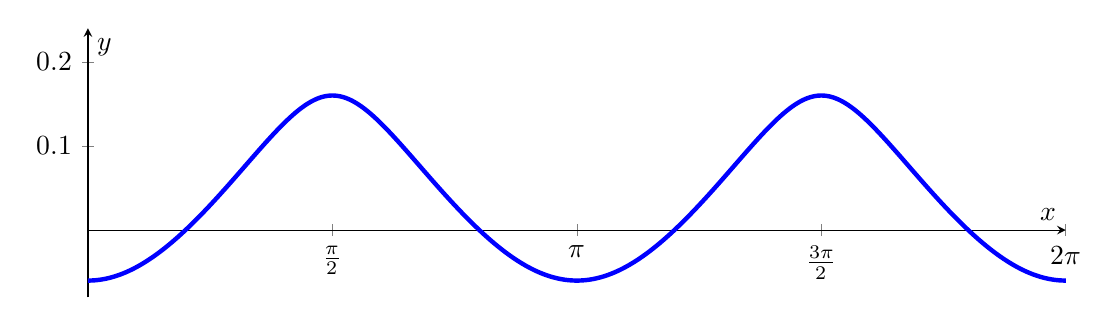
\begin{tikzpicture}
  \begin{axis}[
    axis lines=middle,
    xlabel={$x$},
    ylabel={$y$},
    domain=0:2*pi,
    samples=1200,
    smooth,
    width=14cm,
    height=5cm,
    xmin=0,
    xmax=2*pi,
    ymin=-0.08,
    ymax=0.24,
    xtick={0,1.5708,3.14159,4.71239,6.28318},
    xticklabels={$0$, $\frac{\pi}{2}$, $\pi$, $\frac{3\pi}{2}$, $2\pi$},
  ]

    % Gerstner-like wave with softer crests
    \addplot[
      blue,
      ultra thick,
      variable=\t,
      parametric
    ]
    (
      {
        \t
        + 0.10*sin(deg(2*\t))
        - 0.015*sin(deg(4*\t))
      },
      {
        0.11*(1 - cos(deg(2*\t)))
        - 0.06
      }
    );

  \end{axis}
\end{tikzpicture}
\caption{Κύμα Gerstner.}
\label{fig:gerstner}
\end{figure}

Κάθε σημείο της επιφάνειας δίνεται παραμετρικά από τις ακόλουθες
εξισώσεις. Η ιδέα αυτή εφαρμόστηκε πρώτη φορά στα γραφικά από τους
Fournier \& Reeves (Fournier and Reeves 1986) και αποτέλεσε τη βάση για
την ακριβή διατύπωση του Tessendorf (Tessendorf 2001):

\begin{itemize}
\tightlist
\item
  \(x(u, t) = u - \frac{A k}{|k|} \sin(k u - \omega t + \varphi)\)
\item
  \(y(u, t) = A \cos(k u - \omega t + \varphi)\)
\end{itemize}

όπου \(u\) είναι η αρχική οριζόντια θέση του σημείου στην επιφάνεια
ηρεμίας (όταν δεν υπάρχει κύμα). Σε αντίθεση με το ημιτονοειδές κύμα,
όπου κάθε σημείο ταλαντώνεται κατακόρυφα γύρω από σταθερή οριζόντια
θέση, εδώ το σημείο διαγράφει κυκλική τροχιά, εκτρέποντας οριζόντια την
επιφάνεια.

Παράμετροι:

\begin{itemize}
\tightlist
\item
  \(A\) (πλάτος): Ακτίνα της κυκλικής τροχιάς.
\item
  \(k\) (κυματαριθμός): \(k = \frac{2\pi}{\lambda}\). Για \(k>0\) ο όρος
  \(\frac{A k}{|k|}\) απλοποιείται σε \(A\)· το πρόσημο του \(k\)
  καθορίζει την κατεύθυνση διάδοσης.
\item
  \(\omega\) (γωνιακή συχνότητα): \(\omega = \sqrt{g k}\) (σχέση
  διασποράς, όπου \(g\approx 9.81\,\text{m/s}^2\) η επιτάχυνση της
  βαρύτητας).
\item
  \(\varphi\) (αρχική φάση): Οριζόντια μετατόπιση.
\end{itemize}

\begin{figure}[htbp]
\centering
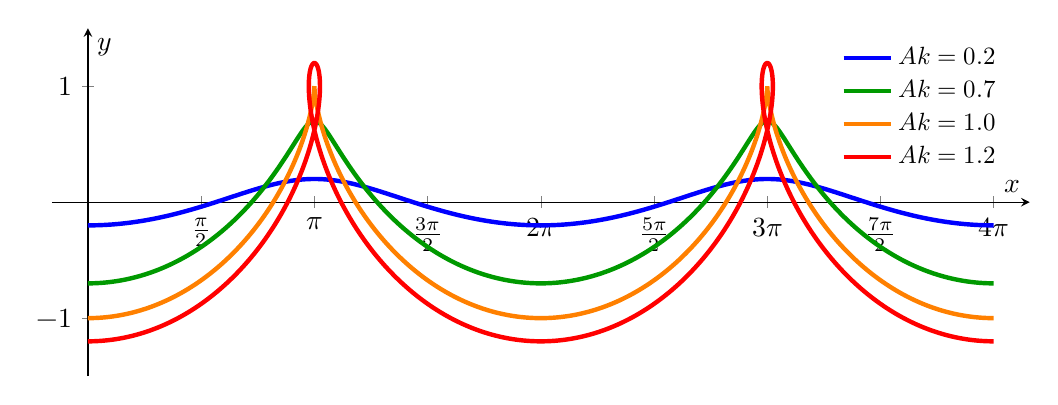
\begin{tikzpicture}
  \begin{axis}[
    axis lines=middle,
    xlabel={$x$},
    ylabel={$y$},
    domain=0:4*pi,
    samples=500,
    smooth,
    width=14cm,
    height=6cm,
    xmin=-0.5,
    xmax=4*pi+0.5,
    ymin=-1.5,
    ymax=1.5,
    xtick={0,1.5708,3.14159,4.71239,6.28318,7.85398,9.42478,10.9956,12.5664},
    xticklabels={$0$, $\frac{\pi}{2}$, $\pi$, $\frac{3\pi}{2}$, $2\pi$, $\frac{5\pi}{2}$, $3\pi$, $\frac{7\pi}{2}$, $4\pi$},
    legend style={at={(0.98,0.98)}, anchor=north east, draw=none, font=\small}
  ]

    % A = 0.2
    \addplot[
      blue,
      ultra thick,
      variable=\t,
      parametric
    ]
    (
      {
        \t + 0.2*sin(deg(\t))
      },
      {
        -0.2*cos(deg(\t))
      }
    );
    \addlegendentry{$A k = 0.2$}

    % A = 0.7
    \addplot[
      green!60!black,
      ultra thick,
      variable=\t,
      parametric
    ]
    (
      {
        \t + 0.7*sin(deg(\t))
      },
      {
        -0.7*cos(deg(\t))
      }
    );
    \addlegendentry{$A k = 0.7$}

    % A = 1.0
    \addplot[
      orange,
      ultra thick,
      variable=\t,
      parametric
    ]
    (
      {
        \t + 1.0*sin(deg(\t))
      },
      {
        -1.0*cos(deg(\t))
      }
    );
    \addlegendentry{$A k = 1.0$}

    % A = 1.2
    \addplot[
      red,
      ultra thick,
      variable=\t,
      parametric
    ]
    (
      {
        \t + 1.2*sin(deg(\t))
      },
      {
        -1.2*cos(deg(\t))
      }
    );
    \addlegendentry{$A k = 1.2$}

  \end{axis}
\end{tikzpicture}
\caption{Επίδραση του γινομένου $A k$ στη μορφή των κυμάτων Gerstner.}
\label{fig:gerstner_ak}
\end{figure}

Ιδιαίτερη προσοχή πρέπει να δοθεί στην περίπτωση \(A \cdot k > 1\)
(Σχήμα \ref{fig:gerstner_ak}), όπου η επιφάνεια αναδιπλώνεται
δημιουργώντας βρόχους, κάτι φυσικά αδύνατο για ένα υγρό. Για ρεαλιστικές
προσομοιώσεις, απαιτείται \(A \cdot k < 1\).

\subsection{Άθροισμα
συχνοτήτων}\label{ux3acux3b8ux3c1ux3bfux3b9ux3c3ux3bcux3b1-ux3c3ux3c5ux3c7ux3bdux3bfux3c4ux3aeux3c4ux3c9ux3bd}

Η υπέρθεση πολλών ημιτονοειδών κυμάτων με διαφορετικά πλάτη, συχνότητες
και φάσεις παράγει σύνθετα σήματα. Η προσθήκη περισσότερων συνιστωσών
επιτρέπει την προσέγγιση σχεδόν οποιασδήποτε περιοδικής κυματομορφής ---
μια ιδέα που αποτελεί τη βάση για τους μετασχηματισμούς Fourier.

\begin{figure}[htbp]
\centering
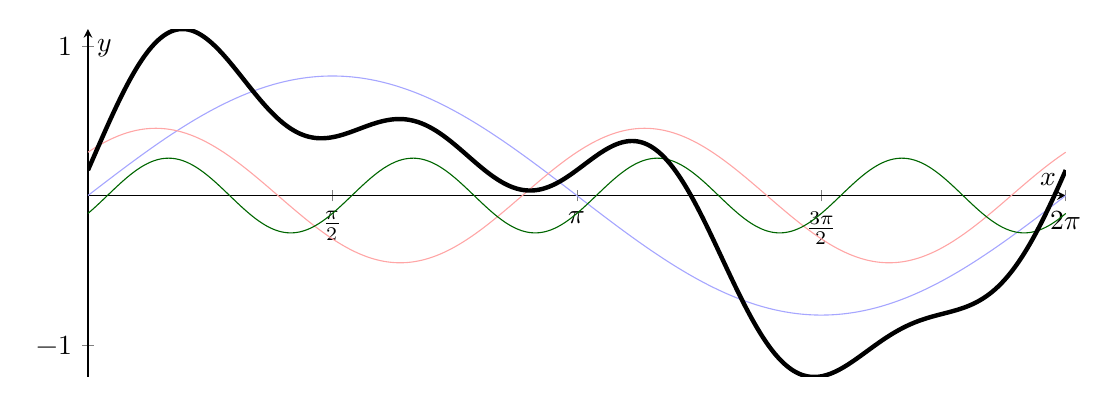
\begin{tikzpicture}
  \begin{axis}[
    domain=0:2*pi,
    samples=400,
    axis lines=middle,
    xlabel={$x$},
    ylabel={$y$},
    width=14cm,
    height=6cm,
    xmin=0,
    xmax=2*pi,
    xtick={0,1.5708,3.14159,4.71239,6.28318},
    xticklabels={$0$, $\frac{\pi}{2}$, $\pi$, $\frac{3\pi}{2}$, $2\pi$},
    legend style={
      at={(0.98,0.98)},
      anchor=north east,
      draw=none
    }
  ]

    % Individual components (faint)
    \addplot[
      blue!35,
      thin
    ]
    {0.8*sin(deg(x))};

    \addplot[
      red!35,
      thin
    ]
    {0.45*sin(deg(2*x + 0.7))};

    \addplot[
      green!40!black,
      thin
    ]
    {0.25*sin(deg(4*x - 0.5))};

    % Superposition (bold)
    \addplot[
      black,
      ultra thick
    ]
    {
      0.8*sin(deg(x))
      + 0.45*sin(deg(2*x + 0.7))
      + 0.25*sin(deg(4*x - 0.5))
    };


  \end{axis}
\end{tikzpicture}
\caption{
Υπέρθεση διάφορων ημιτονοειδών κυμάτων.
}
\label{fig:fourier_superposition}
\end{figure}

\section{Ήχος}\label{ux3aeux3c7ux3bfux3c2}

Η μαθηματική δομή που αναπτύχθηκε για τα κύματα εμφανίζεται αυτούσια και
στον ήχο: οι μεταβολές της πίεσης του αέρα διαδίδονται ως περιοδικές
ταλαντώσεις, και κάθε σύνθετο ακουστικό σήμα μπορεί να αναλυθεί σε
άθροισμα απλών ημιτονοειδών κυμάτων. Το ανθρώπινο αυτί, αλλά και κάθε
μικρόφωνο, λειτουργεί στην πράξη ως ένας φυσικός αναλυτής Fourier,
αποσυνθέτοντας τον ήχο στις συχνότητες που τον αποτελούν (Békésy 1960).

\subsection{Ηχητικό
κύμα}\label{ux3b7ux3c7ux3b7ux3c4ux3b9ux3baux3cc-ux3baux3cdux3bcux3b1}

Ο ήχος αποτελεί ένα οικείο ανάλογο φαινόμενο των κυμάτων νερού, με τη
θεμελιώδη διαφορά ότι, ενώ η επιφάνεια της θάλασσας ταλαντώνεται κυρίως
κάθετα (εγκάρσιο κύμα), στον ήχο τα μόρια του αέρα ταλαντώνονται
παράλληλα προς τη διεύθυνση διάδοσης (διαμήκες κύμα). Ένας καθαρός τόνος
περιγράφεται από την εξίσωση \(p(t) = A \sin(2\pi f t + \varphi)\), όπου
\(p(t)\) είναι η στιγμιαία απόκλιση της ατμοσφαιρικής πίεσης, \(f\) η
συχνότητα (μετρούμενη σε Hz), \(A\) το πλάτος το οποίο σχετίζεται με την
ένταση του ήχου (η ένταση είναι ανάλογη του \(A^2\) και μετριέται σε
ντεσιμπέλ (dB)) και \(\varphi\) η αρχική φάση. Κατά τη διάδοση,
δημιουργούνται διαδοχικές πυκνώσεις (περιοχές υψηλότερης πίεσης) και
αραιώσεις (περιοχές χαμηλότερης πίεσης), οι οποίες μεταφέρουν την
ακουστική ενέργεια.

Η μαθηματική σύνδεση με τα κύματα νερού είναι άμεση: όπως το ύψος μιας
θαλάσσιας επιφάνειας γράφεται ως
\(y(x,t) = A\sin(kx - \omega t + \varphi)\), έτσι και η ηχητική πίεση
γράφεται ως \(p(t) = A\sin(\omega t + \varphi)\), όπου
\(\omega = 2\pi f\). Και στις δύο περιπτώσεις, η θεμελιώδης έννοια είναι
η ταλάντωση γύρω από μια θέση ισορροπίας και η δυνατότητα υπέρθεσης
πολλών ανεξάρτητων ημιτονοειδών συνιστωσών.

\begin{figure}[htbp]
\centering

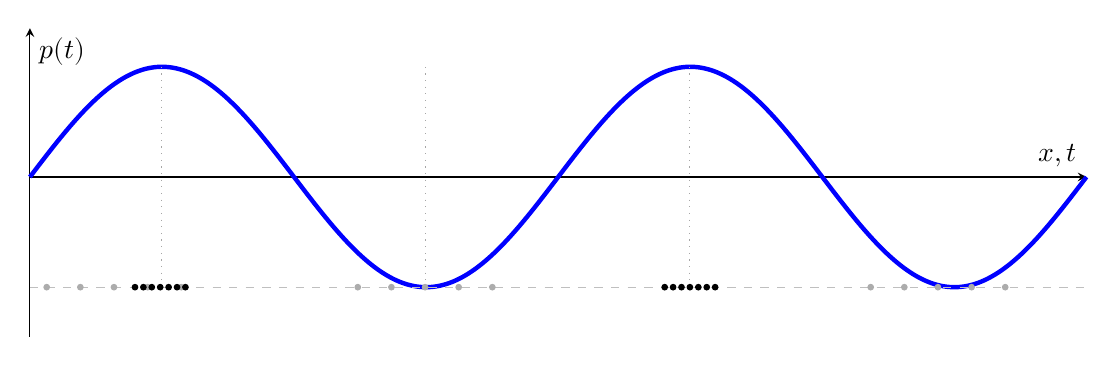
\begin{tikzpicture}

\begin{axis}[
    width=15cm,
    height=5.5cm,
    xmin=0,
    xmax=4*pi,
    ymin=-1.45,
    ymax=1.35,
    axis lines=middle,
    xlabel={$x,t$},
    ylabel={$p(t)$},
    xtick=\empty,
    ytick=\empty,
    samples=600,
    domain=0:4*pi,
    clip=false
]

% =====================================
% SOUND WAVE
% =====================================

\addplot[
    ultra thick,
    blue
]
{sin(deg(x))};

% =====================================
% MOLECULE BASELINE
% =====================================

\addplot[
    dashed,
    gray!50
]
coordinates {(0,-1) (12.57,-1)};

% =====================================
% MOLECULES
% =====================================

% --- rarefaction ---
\addplot[
    only marks,
    mark=*,
    mark size=1pt,
    gray!65
]
coordinates {
(0.2,-1)
(0.6,-1)
(1.0,-1)
(1.4,-1)
(1.8,-1)
};

% --- compression at crest pi/2 ---
\addplot[
    only marks,
    mark=*,
    mark size=1pt,
    black
]
coordinates {
(1.25,-1)
(1.35,-1)
(1.45,-1)
(1.55,-1)
(1.65,-1)
(1.75,-1)
(1.85,-1)
};

% --- rarefaction at trough 3pi/2 ---
\addplot[
    only marks,
    mark=*,
    mark size=1pt,
    gray!65
]
coordinates {
(3.9,-1)
(4.3,-1)
(4.7,-1)
(5.1,-1)
(5.5,-1)
};

% --- compression at crest 5pi/2 ---
\addplot[
    only marks,
    mark=*,
    mark size=1pt,
    black
]
coordinates {
(7.55,-1)
(7.65,-1)
(7.75,-1)
(7.85,-1)
(7.95,-1)
(8.05,-1)
(8.15,-1)
};

% --- rarefaction ---
\addplot[
    only marks,
    mark=*,
    mark size=1pt,
    gray!65
]
coordinates {
(10.0,-1)
(10.4,-1)
(10.8,-1)
(11.2,-1)
(11.6,-1)
};

% ALIGNMENT LINES

\draw[dotted, gray!70]
(axis cs:1.57,1)
--
(axis cs:1.57,-1);

\draw[dotted, gray!70]
(axis cs:4.71,1)
--
(axis cs:4.71,-1);

\draw[dotted, gray!70]
(axis cs:7.85,1)
--
(axis cs:7.85,-1);

\end{axis}

\end{tikzpicture}

\caption{
Συσχέτιση ηχητικής πίεσης και κατανομής μορίων αέρα.
}
\label{fig:soundwave}
\end{figure}

\subsection{Σύνθεση ήχου από πολλαπλές
συχνότητες}\label{ux3c3ux3cdux3bdux3b8ux3b5ux3c3ux3b7-ux3aeux3c7ux3bfux3c5-ux3b1ux3c0ux3cc-ux3c0ux3bfux3bbux3bbux3b1ux3c0ux3bbux3adux3c2-ux3c3ux3c5ux3c7ux3bdux3ccux3c4ux3b7ux3c4ux3b5ux3c2}

Ακριβώς όπως ένα σύνθετο θαλάσσιο κύμα προκύπτει από την άθροιση πολλών
κυματικών συνιστωσών, έτσι και ένας σύνθετος ήχος προκύπτει από την
υπέρθεση επιμέρους τόνων. Αν διαθέτουμε \(N\) ηχητικές πηγές, η καθεμία
με συχνότητα \(f_i\), πλάτος \(A_i\) και φάση \(\varphi_i\), το συνολικό
σήμα είναι

\[
p_{\text{total}}(t) = \sum_{i=1}^{N} A_i \sin(2\pi f_i t + \varphi_i).
\]

Αυτή η γραμμική υπέρθεση είναι η βάση της σύνθεσης Fourier. Σε αντίθεση
με τη θάλασσα, όπου οι συνιστώσες είναι χωρικές συχνότητες
\((k_x, k_z)\), στον ήχο οι συνιστώσες είναι χρονικές συχνότητες \(f\).
Ωστόσο, η μαθηματική δομή είναι ταυτόσημη: κάθε περιοδικό φαινόμενο
μπορεί να αναλυθεί σε άθροισμα ημιτόνων, και η κατανομή των πλατών
\(A_i\) σε συνάρτηση με τη συχνότητα ονομάζεται φάσμα πλάτους, ενώ η
αντίστοιχη κατανομή των φάσεων \(\varphi_i\) ονομάζεται φάσμα φάσης.
Μαζί, τα δύο φάσματα περιγράφουν πλήρως το σήμα.

Οπτικά, η κυματομορφή στο πεδίο του χρόνου δείχνει τη διακύμανση της
πίεσης, ενώ το φάσμα πλάτους εμφανίζει ράβδους ύψους \(A_i\) στις θέσεις
\(f_i\). Η αντιστοιχία αυτή είναι ανάλογη με τη μετάβαση από την
αναπαράσταση \(h(x,z,t)\) (στον φυσικό χώρο) στην αναπαράσταση
\(H(k_x,k_z,t)\) (στο πεδίο των συχνοτήτων) που θα συναντήσουμε στην
προσομοίωση της θάλασσας.

\subsection{Αναλύοντας έναν σύνθετο ήχο στις συνιστώσες
του}\label{ux3b1ux3bdux3b1ux3bbux3cdux3bfux3bdux3c4ux3b1ux3c2-ux3adux3bdux3b1ux3bd-ux3c3ux3cdux3bdux3b8ux3b5ux3c4ux3bf-ux3aeux3c7ux3bf-ux3c3ux3c4ux3b9ux3c2-ux3c3ux3c5ux3bdux3b9ux3c3ux3c4ux3ceux3c3ux3b5ux3c2-ux3c4ux3bfux3c5}

\begin{figure}[htbp]
\centering
\begin{minipage}{0.56\textwidth}
  \centering
  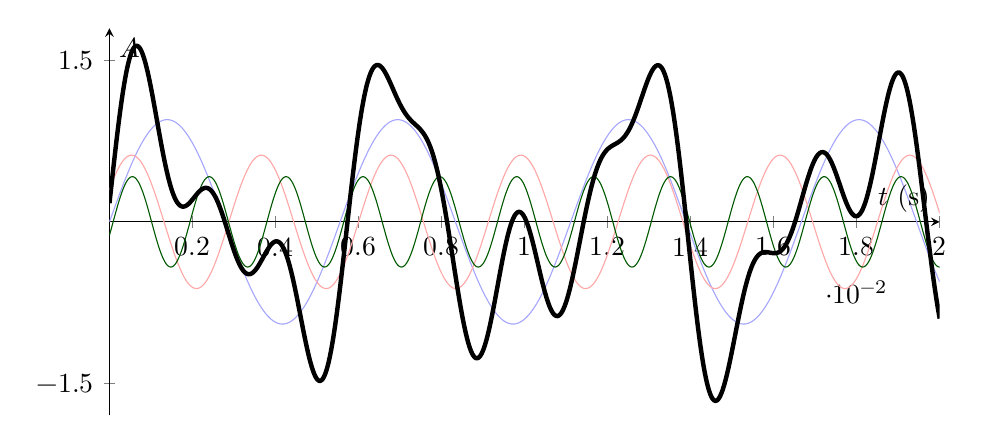
\begin{tikzpicture}
    \begin{axis}[
      width=\textwidth,
      height=6.5cm,
      xlabel={$t$ (s)},
      ylabel={$A$},
      domain=0:0.02,          
      samples=800,          
      axis lines=middle,
      trig format plots=rad,
      % xtick={0,0.02,0.04,0.06,0.08,0.10,0.12,0.14,0.16},
      ytick={-1.5,0,1.5},
      ymin=-1.8, ymax=1.8,
    ]
      \addplot[blue!35, thin] {0.95*sin(2*pi*180*x)};
      \addplot[red!35, thin] {0.62*sin(2*pi*320*x+0.5)};
      \addplot[green!35!black, thin] {0.42*sin(2*pi*540*x-0.3)};
      \addplot[black, ultra thick] {
        0.95*sin(2*pi*180*x) + 0.62*sin(2*pi*320*x+0.5) + 0.42*sin(2*pi*540*x-0.3)
      };
    \end{axis}
  \end{tikzpicture}
\end{minipage}
\hfill
\begin{minipage}{0.40\textwidth}
  \centering
  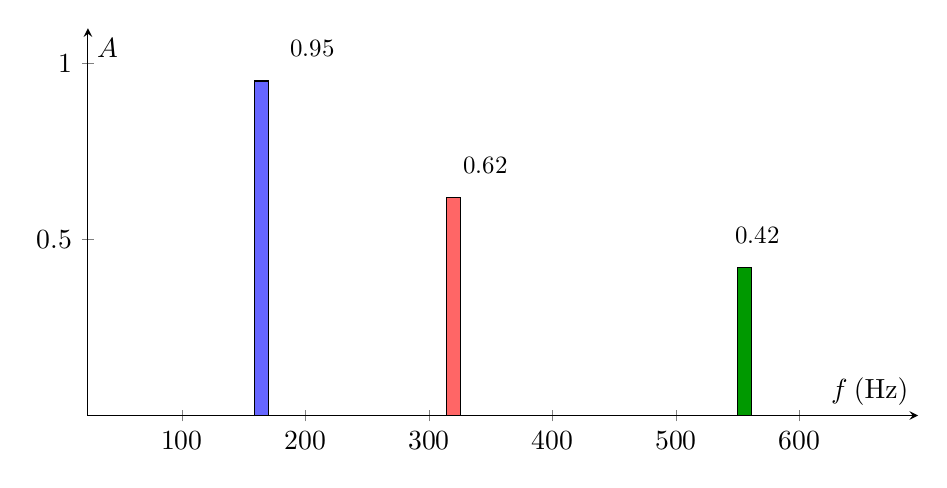
\begin{tikzpicture}
    \begin{axis}[
      width=\textwidth,
      height=6.5cm,
      xlabel={$f$ (Hz)},
      ylabel={$A$},
      ybar,
      bar width=5pt,
      % xtick=data,
      % xticklabels={180,320,540},
      axis lines=middle,
      ymin=0, ymax=1.1,
      xmin=120, xmax=600,
      enlarge x limits=0.2,
      nodes near coords,
      every node near coord/.style={
        anchor=south west,
        yshift=5pt,
        font=\small,
        rotate=0
      }
    ]
      \addplot[fill=blue!60] coordinates {(180,0.95)};
      \addplot[fill=red!60] coordinates {(320,0.62)};
      \addplot[fill=green!60!black] coordinates {(540,0.42)};
    \end{axis}
  \end{tikzpicture}
\end{minipage}
\caption{Σύνθετο κύμα και ανάλυση σε συνιστώσες συχνοτήτων.}
\label{fig:sound_spectrum_analysis}
\end{figure}

Στην πράξη, αν διαθέτουμε ένα σύνθετο σήμα (π.χ. άθροισμα τριών
ημιτόνων), υπάρχει μαθηματική διαδικασία που αποκαλύπτει ακριβώς τις
συχνότητες, τα πλάτη και τις φάσεις που το αποτελούν. Οπτικά, το φάσμα
του σύνθετου σήματος δεν είναι τίποτα άλλο από την ένωση των φασμάτων
των επιμέρους συνιστωσών, ενώ η κυματομορφή στο πεδίο του χρόνου είναι η
υπέρθεσή τους. Έτσι, η σύνθεση (χτίσιμο ενός σύνθετου κύματος από απλά
ημίτονα) και η ανάλυση (αποσύνθεση ενός σύνθετου κύματος στα απλά
ημίτονα που το αποτελούν) αποδεικνύονται δύο όψεις του ίδιου μηχανισμού.
Αυτή ακριβώς η δυαδικότητα θα αποτελέσει τον πυρήνα του μετασχηματισμού
Fourier, ο οποίος με τη σειρά του θα μας επιτρέψει να περάσουμε από τα
ηχητικά σήματα στην ταχύτατη ψηφιακή επεξεργασία και, αργότερα, στην
προσομοίωση του ωκεανού.

\section{Ανάπτυγμα
Taylor}\label{ux3b1ux3bdux3acux3c0ux3c4ux3c5ux3b3ux3bcux3b1-taylor}

Τόσο στα κύματα νερού όσο και στον ήχο, οι συναρτήσεις που εμφανίζονται
συχνότερα είναι οι ημιτονοειδείς. Για έναν υπολογιστή, ωστόσο, ο
απευθείας υπολογισμός τους είναι αριθμητικά απαιτητικός. Θα ήταν πολύ
πιο βολικό να τις αντικαταστήσουμε με πολυώνυμα -- αθροίσματα όρων
\(a_n x^n\) -- που χρησιμοποιούν μόνο προσθέσεις, αφαιρέσεις και
πολλαπλασιασμούς, δηλαδή πράξεις πολύ γρήγορες για τον επεξεργαστή.
Ακριβώς αυτό επιτυγχάνει το ανάπτυγμα Taylor, το οποίο εισήγαγε ο Brook
Taylor το 1715 (Taylor 1715) και παραμένει θεμελιώδες εργαλείο στην
αριθμητική ανάλυση (Burden and Faires 2016). Η σειρά Taylor λειτουργεί
ως εξής: κοντά σε ένα σημείο \(x_0\), μια ομαλή συνάρτηση \(f(x)\)
μπορεί να προσεγγιστεί από ένα πολυώνυμο του οποίου οι συντελεστές
καθορίζονται από τις παραγώγους της \(f\) στο \(x_0\). Αν γνωρίζουμε την
τιμή \(f(x_0)\), την κλίση \(f'(x_0)\), την καμπυλότητα \(f''(x_0)\)
κ.ο.κ., τότε το πολυώνυμο
\[ f(x) \approx f(x_0) + f'(x_0)(x-x_0) + \frac{f''(x_0)}{2}(x-x_0)^2 + \cdots + \frac{f^{(n)}(x_0)}{n!}(x-x_0)^n \]
πλησιάζει την \(f(x)\) όλο και καλύτερα όσο αυξάνουμε τον αριθμό των
όρων \(n\). Στο όριο άπειρων όρων, υπό προϋποθέσεις παίρνουμε την ακριβή
αναπαράσταση, γνωστή ως σειρά Taylor. Αν και το ανάπτυγμα Taylor είναι
το θεωρητικό θεμέλιο, οι σύγχρονοι υπολογιστές χρησιμοποιούν συχνά
βελτιστοποιημένες πολυωνυμικές προσεγγίσεις (π.χ. ελαχίστου σφάλματος)
για ακόμα μεγαλύτερη ακρίβεια σε όλο το εύρος τιμών.

Για μια ευρεία κλάση συναρτήσεων, γνωστών ως αναλυτικών, η σειρά Taylor
συγκλίνει στην ίδια τη συνάρτηση σε μια περιοχή γύρω από το σημείο
ανάπτυξης. Στην κλάση αυτή ανήκουν το ημίτονο (\(\sin x\)), το
συνημίτονο (\(\cos x\)) και η εκθετική συνάρτηση (\(e^x\)) καθώς και
κάθε γραμμικός συνδυασμός ή γινόμενο αυτών. Για τις συναρτήσεις αυτές, η
ακτίνα σύγκλισης είναι \(R = \infty\), δηλαδή η σειρά συγκλίνει για κάθε
πραγματικό \(x\). Ακόμη και με πεπερασμένο αριθμό όρων, η προσέγγιση
είναι εξαιρετική κοντά στο σημείο ανάπτυξης, γεγονός που αξιοποιείται
από όλες τις σύγχρονες μαθηματικές βιβλιοθήκες.

Η εφαρμογή της σειράς Taylor σε τρεις χαρακτηριστικές συναρτήσεις -- το
ημίτονο, το συνημίτονο και την εκθετική -- καθώς και σε έναν γραμμικό
συνδυασμό τους, εξετάζεται στη συνέχεια. Το πρώτο παράδειγμα είναι η
συνάρτηση \(e^{x/2}\cos(x)\).

\subsection{\texorpdfstring{Ανάπτυγμα της
\(e^{x/2}\cos(x)\)}{Ανάπτυγμα της e\^{}\{x/2\}\textbackslash cos(x)}}\label{ux3b1ux3bdux3acux3c0ux3c4ux3c5ux3b3ux3bcux3b1-ux3c4ux3b7ux3c2-ex2cosx}

Η καλύτερη γραμμική προσέγγιση μιας συνάρτησης σε ένα σημείο είναι
εκείνη για την οποία η τιμή και η παράγωγος της προσέγγισης συμπίπτουν
με την τιμή και την παράγωγο της συνάρτησης στο σημείο αυτό.

Για τη συνάρτηση \(f(x) = e^{x/2} \cos(x)\), στο σημείο \(x = 0\)
υπολογίζουμε
\(f'(x) = \frac{1}{2} e^{x/2} \cos(x) - e^{x/2} \sin(x) = e^{x/2} \left( \frac{1}{2} \cos(x) - \sin(x) \right)\),
άρα:

\begin{itemize}
\tightlist
\item
  \(f(0) = e^{0} \cos(0) = 1 \cdot 1 = 1\),\\
\item
  \(f'(0) = e^{0} \left( \frac{1}{2} \cdot 1 - 0 \right) = \frac{1}{2}\).
\end{itemize}

Επομένως, η γραμμική προσέγγιση (πολυώνυμο Taylor πρώτου βαθμού) είναι:

\[
\boxed{T_1(x) = f(0) + f'(0) \, x = 1 + \frac{x}{2}}.
\]

\begin{figure}[htbp]
\centering
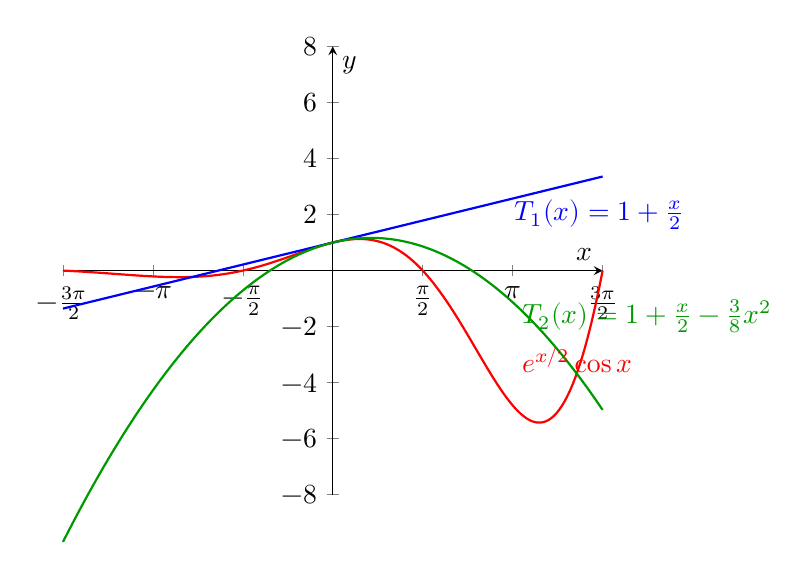
\begin{tikzpicture}
  \begin{axis}[
    trig format plots=rad,
    axis lines=middle,
    xlabel={$x$},
    ylabel={$y$},
    domain=-1.5*pi:1.5*pi,
    samples=300,
    ymin=-8,
    ymax=8,
    clip=false,
    xtick={-6.28318, -4.71239, -3.14159, -1.5708, 0, 1.5708, 3.14159, 4.71239, 6.28318},
    xticklabels={$-2\pi$, $-\frac{3\pi}{2}$, $-\pi$, $-\frac{\pi}{2}$, $0$, $\frac{\pi}{2}$, $\pi$, $\frac{3\pi}{2}$, $2\pi$},
    ytick={-8,-6,-4,-2,0,2,4,6,8},
  ]
    % Αρχική συνάρτηση
    \addplot[red, thick] {exp(x/2)*cos(x)};
    % Γραμμική προσέγγιση T1(x)
    \addplot[blue, thick] {1 + 0.5*x};
    % Τετραγωνική προσέγγιση T2(x)
    \addplot[green!60!black, thick, domain=-1.5*pi:1.5*pi] {1 + 0.5*x - 0.375*x^2};
    
    \node[red, anchor=west] at (axis cs:3.14, {exp(3.14/2)*cos(3.14)-8}) {$e^{x/2}\cos x$};
    \node[blue, anchor=west] at (axis cs:3., {1 + 0.5*3.-0.5}) {$T_1(x)=1+\frac{x}{2}$};
    \node[green!60!black, anchor=west] at (axis cs:3.14, {1 + 0.5*3.14 - 0.375*3.14^2 - 0.5}) {$T_2(x)=1+\frac{x}{2}-\frac{3}{8}x^2$};
  \end{axis}
\end{tikzpicture}
\caption{Σύγκριση $e^{x/2}\cos x$ με τις προσεγγίσεις Taylor $T_1(x)$ και $T_2(x)$.}
\label{fig:expcoslinear}
\end{figure}

Παραγωγίζοντας ξανά, προκύπτει: \[
f''(x) =  e^{x/2} \left( -\frac{3}{4}\cos x - \sin x \right),
\] οπότε στο \(x=0\): \[
f''(0) = e^{0} \left( -\frac{3}{4} \cdot 1 - 0 \right) = -\frac{3}{4}.
\]

Έτσι, η τετραγωνική προσέγγιση (πολυώνυμο Taylor δεύτερου βαθμού) είναι:

\[
\boxed{T_2(x) = f(0) + f'(0)\,x + \frac{f''(0)}{2}\,x^2 = 1 + \frac{x}{2} - \frac{3}{8}x^2}.
\]

Σημειώνεται ότι, ενώ η δεύτερη παράγωγος της συνάρτησης στο \(0\) είναι
\(-\frac{3}{4}\), για έναν όρο \(a x^2\) στο πολυώνυμο ισχύει
\(\frac{d^2}{dx^2}(a x^2)=2a\). Άρα, αφού \(P''(0)=2a=-\frac{3}{4}\),
προκύπτει \(a=-\frac{3}{8}\).

Αν η διαδικασία συνεχιστεί, κάθε πολυώνυμο μεγαλύτερου βαθμού
ενσωματώνει περισσότερη πληροφορία, οδηγώντας σε ολοένα καλύτερη
προσέγγιση. Η αναπαράσταση μιας συνάρτησης ως άπειρο άθροισμα
πολυωνυμικών όρων ονομάζεται σειρά Taylor.

\begin{figure}[htbp]
\centering
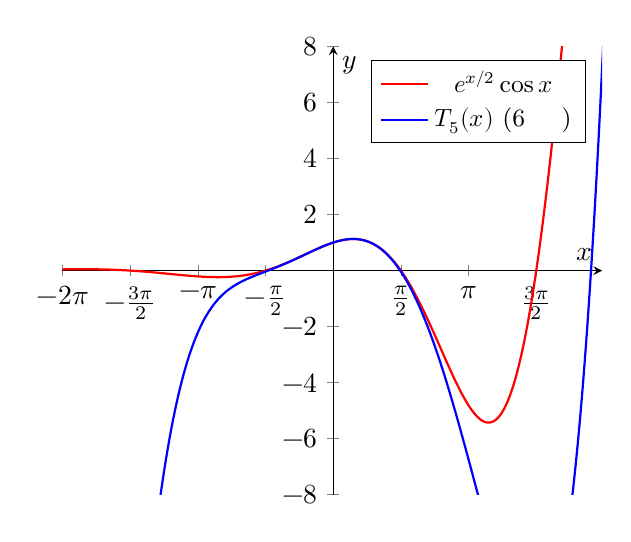
\begin{tikzpicture}
  \begin{axis}[
    trig format plots=rad,
    axis lines=middle,
    xlabel={$x$},
    ylabel={$y$},
    domain=-2*pi:2*pi,
    samples=300,
    ymin=-8,
    ymax=8,
    xtick={-6.28318, -4.71239, -3.14159, -1.5708, 0, 1.5708, 3.14159, 4.71239, 6.28318},
    xticklabels={$-2\pi$, $-\frac{3\pi}{2}$, $-\pi$, $-\frac{\pi}{2}$, $0$, $\frac{\pi}{2}$, $\pi$, $\frac{3\pi}{2}$, $2\pi$},
    ytick={-8,-6,-4,-2,0,2,4,6,8},
    legend pos=north east,
    legend style={font=\small}
  ]
    \addplot[red, thick] {exp(x/2)*cos(x)};
    \addlegendentry{$e^{x/2}\cos x$}
    
    \addplot[blue, thick] {1 + 0.5*x - 0.375*x^2 - 0.2291666667*x^3 - 0.0182291667*x^4 + 0.0106770833*x^5};
    \addlegendentry{$T_5(x)$ (6 όροι)}
  \end{axis}
\end{tikzpicture}
\caption{Σύγκριση $e^{x/2}\cos x$ με το πολυώνυμο Taylor 5ου βαθμού.}
\label{fig:expcostaylor}
\end{figure}

Ο γενικός τύπος της σειράς γύρω από το \(0\) (ανάπτυγμα Maclaurin)
είναι:

\[f(x) = f(0) + \frac{f'(0)}{1!}x + \frac{f''(0)}{2!}x^2 + \frac{f'''(0)}{3!}x^3 + \dots\]

\subsection{\texorpdfstring{Ανάπτυγμα της
\(\cos(x)\)}{Ανάπτυγμα της \textbackslash cos(x)}}\label{ux3b1ux3bdux3acux3c0ux3c4ux3c5ux3b3ux3bcux3b1-ux3c4ux3b7ux3c2-cosx}

Επειδή η συνάρτηση \(\cos(x)\) είναι άρτια, όλες οι περιττές παράγωγοί
της στο 0 μηδενίζονται. Συνεπώς, στο ανάπτυγμα Maclaurin εμφανίζονται
μόνο άρτιες δυνάμεις του \(x\). Πράγματι, υπολογίζοντας τις παραγώγους:

\begin{itemize}
\tightlist
\item
  \(f(0) = \cos(0) = 1\)
\item
  \(f'(0) = -\sin(0) = 0\)
\item
  \(f''(0) = -\cos(0) = -1\)
\item
  \(f'''(0) = \sin(0) = 0\)
\item
  \(f^{(4)}(0) = \cos(0) = 1\), κ.ο.κ.
\end{itemize}

Αντικαθιστώντας στον τύπο
\(f(x)=\sum_{n=0}^{\infty} \frac{f^{(n)}(0)}{n!}x^n\), προκύπτει:

\[
\cos(x) = 1 - \frac{x^2}{2!} + \frac{x^4}{4!} - \frac{x^6}{6!} + \cdots = \sum_{n=0}^{\infty} (-1)^n \frac{x^{2n}}{(2n)!}
\]

\begin{figure}[htbp]
\centering
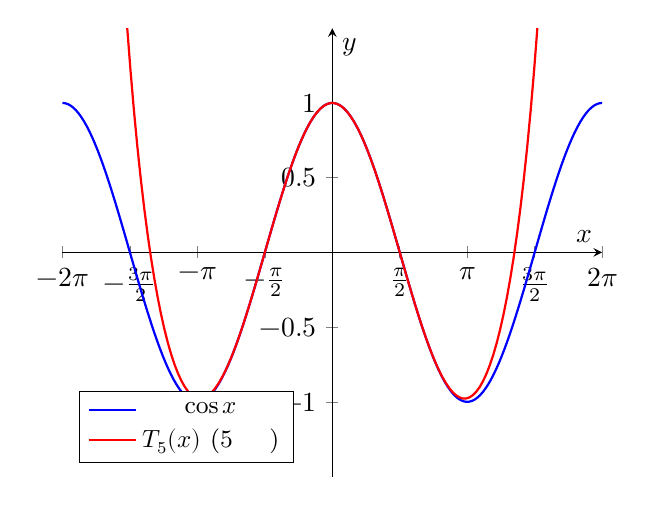
\begin{tikzpicture}
  \begin{axis}[
    trig format plots=rad,
    axis lines=middle,
    xlabel={$x$},
    ylabel={$y$},
    domain=-2*pi:2*pi,
    samples=200,
    ymin=-1.5, ymax=1.5,
    xtick={-6.28318, -4.71239, -3.14159, -1.5708, 0, 1.5708, 3.14159, 4.71239, 6.28318},
    xticklabels={$-2\pi$, $-\frac{3\pi}{2}$, $-\pi$, $-\frac{\pi}{2}$, $0$, $\frac{\pi}{2}$, $\pi$, $\frac{3\pi}{2}$, $2\pi$},
    ytick={-1, -0.5, 0, 0.5, 1},
    legend pos=south west,
    legend style={font=\small}
  ]
    \addplot[blue, thick] {cos(x)};
    \addlegendentry{$\cos x$}
    
    \addplot[red, thick, domain=-2.5*pi:2.5*pi] {1 - x^2/2 + x^4/24 - x^6/720 + x^8/40320};
    \addlegendentry{$T_5(x)$ (5 όροι)}
  \end{axis}
\end{tikzpicture}
\caption{Σύγκριση $\cos x$ με το πολυώνυμο Taylor 5 όρων (έως $x^8$).}
\label{fig:costaylor5}
\end{figure}

Στο σχήμα \ref{fig:costaylor5} ο δείκτης μετρά τους μη-μηδενικούς όρους,
όχι τον βαθμό, αφού οι περιττές δυνάμεις μηδενίζονται.

\subsection{\texorpdfstring{Ανάπτυγμα της
\(\sin(x)\)}{Ανάπτυγμα της \textbackslash sin(x)}}\label{ux3b1ux3bdux3acux3c0ux3c4ux3c5ux3b3ux3bcux3b1-ux3c4ux3b7ux3c2-sinx}

Το \(\sin(x)\) είναι περιττή συνάρτηση, οπότε το ανάπτυγμα περιέχει μόνο
περιττές δυνάμεις. Οι παράγωγοι στο \(0\) δίνουν:

\begin{itemize}
\tightlist
\item
  \(\sin(0)=0\)
\item
  \(\cos(0)=1\)
\item
  \(-\sin(0)=0\)
\item
  \(-\cos(0)=-1\)
\item
  \(\sin(0)=0\), \(\dots\)
\end{itemize}

Έτσι:

\[
\sin(x) = x - \frac{x^3}{3!} + \frac{x^5}{5!} - \frac{x^7}{7!} + \cdots = \sum_{n=0}^{\infty} (-1)^n \frac{x^{2n+1}}{(2n+1)!}
\]

Παρατηρούμε ότι η σειρά του \(\cos(x)\) είναι η παράγωγος όρο προς όρο
της σειράς του \(\sin(x)\), συμφωνώντας με \((\sin x)' = \cos x\).

\begin{figure}[htbp]
\centering
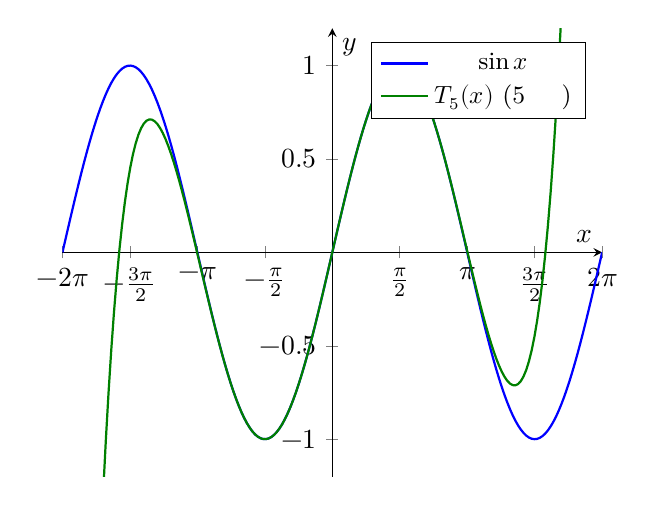
\begin{tikzpicture}
  \begin{axis}[
    trig format plots=rad,
    axis lines=middle,
    xlabel={$x$},
    ylabel={$y$},
    domain=-2*pi:2*pi,
    samples=200,
    ymin=-1.2,
    ymax=1.2,
    xtick={-6.28318, -4.71239, -3.14159, -1.5708, 0, 1.5708, 3.14159, 4.71239, 6.28318},
    xticklabels={$-2\pi$, $-\frac{3\pi}{2}$, $-\pi$, $-\frac{\pi}{2}$, $0$, $\frac{\pi}{2}$, $\pi$, $\frac{3\pi}{2}$, $2\pi$},
    ytick={-1, -0.5, 0, 0.5, 1},
    legend pos=north east,
    legend style={font=\small}
  ]
    \addplot[blue, thick, domain=-2*pi:2*pi] {sin(x)};
    \addlegendentry{$\sin x$}
    
    \addplot[green!50!black, thick, domain=-2*pi:2*pi] {x - x^3/6 + x^5/120 - x^7/5040 + x^9/362880};
    \addlegendentry{$T_5(x)$ (5 όροι)}
  \end{axis}
\end{tikzpicture}
\caption{Σύγκριση $\sin x$ με πολυώνυμο Taylor 5 όρων.}
\label{fig:sintaylor}
\end{figure}

\subsection{\texorpdfstring{Ανάπτυγμα της
\(e^x\)}{Ανάπτυγμα της e\^{}x}}\label{ux3b1ux3bdux3acux3c0ux3c4ux3c5ux3b3ux3bcux3b1-ux3c4ux3b7ux3c2-ex}

Η εκθετική συνάρτηση \(e^x\) ισούται με κάθε της παράγωγο:
\((e^x)^{(n)} = e^x\). Στο \(x=0\):

\[
f^{(n)}(0) = e^0 = 1 \quad \text{για κάθε } n.
\]

Ο τύπος Maclaurin δίνει:

\[
e^x = 1 + x + \frac{x^2}{2!} + \frac{x^3}{3!} + \frac{x^4}{4!} + \cdots = \sum_{n=0}^{\infty} \frac{x^n}{n!}
\]

\begin{figure}[htbp]
\centering
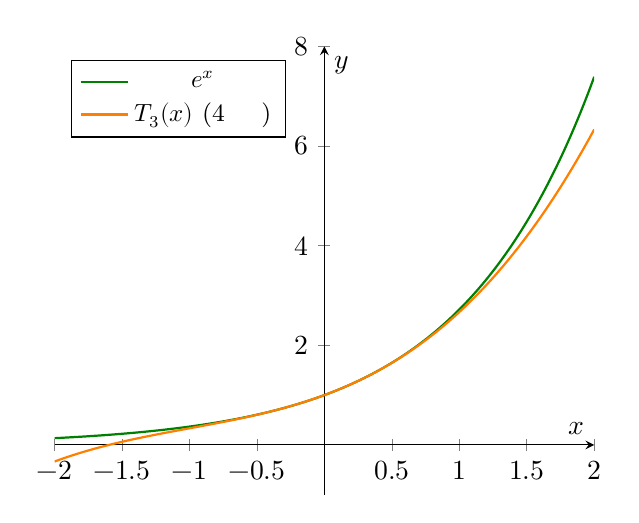
\begin{tikzpicture}
  \begin{axis}[
    axis lines=middle,
    xlabel={$x$},
    ylabel={$y$},
    domain=-2:2,
    samples=200,
    ymin=-1,
    ymax=8,
    xtick={-2,-1.5,-1,-0.5,0,0.5,1,1.5,2},
    ytick={0,2,4,6,8},
    legend pos=north west,
    legend style={font=\small}
  ]
    \addplot[green!50!black, thick] {exp(x)};
    \addlegendentry{$e^x$}
    
    \addplot[orange, thick] {1 + x + x^2/2 + x^3/6};
    \addlegendentry{$T_3(x)$ (4 όροι)}
  \end{axis}
\end{tikzpicture}
\caption{Σύγκριση $e^x$ με το πολυώνυμο Taylor 3ου βαθμού (4 όροι).}
\label{fig:exptaylor}
\end{figure}

\section{Ο τύπος του
Euler}\label{ux3bf-ux3c4ux3cdux3c0ux3bfux3c2-ux3c4ux3bfux3c5-euler}

Οι σειρές Taylor που μόλις αναπτύξαμε για τις συναρτήσεις \(e^x\),
\(\sin x\) και \(\cos x\) δεν είναι απλώς χρήσιμες για αριθμητικές
προσεγγίσεις. Συνδυάζοντάς τες αποκαλύπτουν μια βαθύτερη σχέση που
συνδέει την εκθετική με τις τριγωνομετρικές συναρτήσεις στο μιγαδικό
πεδίο --- τον τύπο του Euler. Θα τον εξάγουμε πρώτα αλγεβρικά, και στη
συνέχεια θα δούμε τη γεωμετρική του ερμηνεία ως περιστροφή.

\subsection{Αλγεβρική απόδειξη (σειρές
Taylor)}\label{ux3b1ux3bbux3b3ux3b5ux3b2ux3c1ux3b9ux3baux3ae-ux3b1ux3c0ux3ccux3b4ux3b5ux3b9ux3beux3b7-ux3c3ux3b5ux3b9ux3c1ux3adux3c2-taylor}

Ξεκινάμε από το ανάπτυγμα της εκθετικής:

\[
e^{x} = \sum_{n=0}^{\infty} \frac{x^n}{n!} = 1 + x + \frac{x^2}{2!} + \frac{x^3}{3!} + \frac{x^4}{4!} + \cdots
\]

Αντικαθιστούμε το \(x\) με το \(ix\) στην παραπάνω σειρά και
χρησιμοποιούμε \(i^2 = -1\), \(i^3 = -i\), \(i^4 = 1\), κ.ο.κ.:

\[
e^{ix} = 1 + ix - \frac{x^2}{2!} - i\frac{x^3}{3!} + \frac{x^4}{4!} + i\frac{x^5}{5!} - \frac{x^6}{6!} - i\frac{x^7}{7!} + \cdots
\]

Ομαδοποιούμε πραγματικούς και φανταστικούς όρους:

\begin{itemize}
\tightlist
\item
  \textbf{Πραγματικοί όροι:}
  \(1 - \frac{x^2}{2!} + \frac{x^4}{4!} - \frac{x^6}{6!} + \cdots = \cos x\)
\item
  \textbf{Φανταστικοί όροι:}
  \(i\left(x - \frac{x^3}{3!} + \frac{x^5}{5!} - \frac{x^7}{7!} + \cdots\right) = i\sin x\)
\end{itemize}

Επομένως:

\[
\boxed{e^{ix} = \cos x + i\sin x}
\]

Αντιστρόφως, λύνοντας το σύστημα των δύο εξισώσεων (για \(x\) και
\(-x\)) ως προς \(\cos x\) και \(\sin x\), προκύπτουν οι εξαιρετικά
χρήσιμες ταυτότητες: \[
\cos x = \frac{e^{ix} + e^{-ix}}{2}, \qquad 
\sin x = \frac{e^{ix} - e^{-ix}}{2i}.
\] Οι σχέσεις αυτές θα αποτελέσουν τον πυρήνα του μετασχηματισμού
Fourier, καθώς επιτρέπουν την έκφραση κάθε ημιτονοειδούς συνιστώσας ως
αθροίσματος δύο μιγαδικών εκθετικών με θετικές και αρνητικές συχνότητες.

\begin{figure}[htbp]
\centering
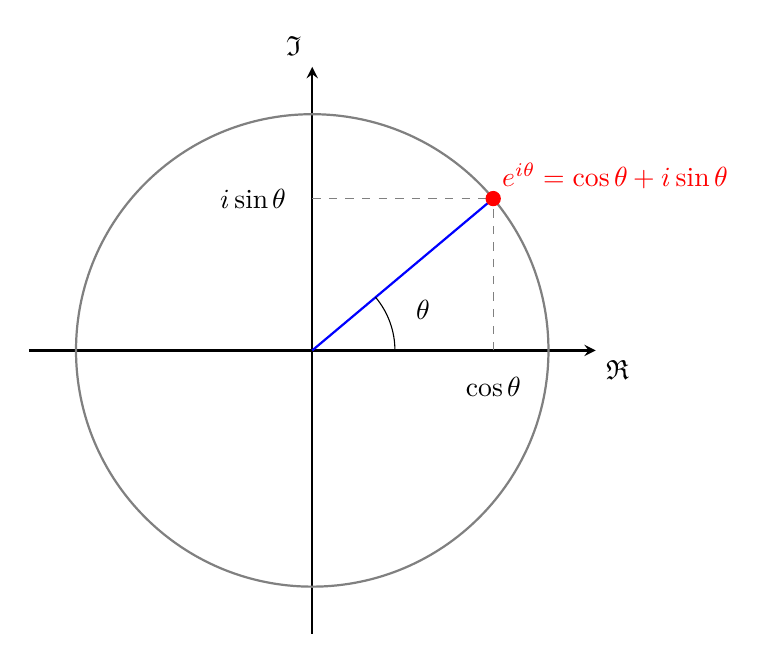
\begin{tikzpicture}[scale=3,>=stealth]
  % Axes
  \draw[->,thick] (-1.2,0) -- (1.2,0) node[below right] {$\Re$};
  \draw[->,thick] (0,-1.2) -- (0,1.2) node[above left] {$\Im$};
  % Unit circle
  \draw[gray, thick] (0,0) circle (1);
  % Angle (40°)
  \def\angle{40}
  % Projections
  \draw[dashed, gray] ({cos(\angle)},0) -- ({cos(\angle)},{sin(\angle)});
  \draw[dashed, gray] (0,{sin(\angle)}) -- ({cos(\angle)},{sin(\angle)});
  % Vector
  \draw[blue, thick] (0,0) -- ({cos(\angle)},{sin(\angle)});
  % Point
  \filldraw[red] ({cos(\angle)},{sin(\angle)}) circle (0.03) 
    node[above right] {$e^{i\theta} = \cos\theta + i\sin\theta$};
  % Arc
  \draw (0.35,0) arc (0:\angle:0.35);
  \node at ({\angle/2}:0.5) {$\theta$};
  % Labels
  \node at ({cos(\angle)}, -0.07) [below] {$\cos\theta$};
  \node at (-0.07, {sin(\angle)}) [left] {$i\sin\theta$};
\end{tikzpicture}
\caption{Μιγαδικό επίπεδο: ο μοναδιαίος κύκλος και η αναπαράσταση του $e^{i\theta}$.}
\label{fig:euler}
\end{figure}

Η παραπάνω ταυτότητα συνδέει την εκθετική με τις τριγωνομετρικές
συναρτήσεις στο μιγαδικό πεδίο και αποτελεί θεμέλιο για τις σειρές
Fourier και την ανάλυση κυματομορφών. Για παράδειγμα, ένα κινούμενο κύμα
της μορφής \(A\sin(kx - \omega t + \varphi)\) μπορεί να γραφεί ως το
φανταστικό μέρος ενός μιγαδικού εκθετικού:

\[
A\sin(kx - \omega t + \varphi) = \operatorname{Im}\left( A e^{i(kx - \omega t + \varphi)} \right).
\]

\subsection{\texorpdfstring{Γεωμετρική ερμηνεία: ο \(i\) ως
περιστροφή}{Γεωμετρική ερμηνεία: ο i ως περιστροφή}}\label{ux3b3ux3b5ux3c9ux3bcux3b5ux3c4ux3c1ux3b9ux3baux3ae-ux3b5ux3c1ux3bcux3b7ux3bdux3b5ux3afux3b1-ux3bf-i-ux3c9ux3c2-ux3c0ux3b5ux3c1ux3b9ux3c3ux3c4ux3c1ux3bfux3c6ux3ae}

Ο τύπος του Euler αποκαλύπτει ότι ο πολλαπλασιασμός ενός μιγαδικού
αριθμού με \(e^{i\theta}\) αντιστοιχεί σε περιστροφή κατά γωνία
\(\theta\) στο μιγαδικό επίπεδο. Πράγματι, αν \(z = r e^{i\varphi}\),
τότε:

\[
z \cdot e^{i\theta} = r e^{i(\varphi + \theta)}.
\]

Το μέτρο \(r\) παραμένει ίδιο, ενώ η γωνία αυξάνεται κατά \(\theta\).
Ειδικότερα, ο πολλαπλασιασμός με \(i = e^{i\pi/2}\) στρέφει ένα διάνυσμα
κατά \(90^\circ\) αριστερόστροφα:

\begin{itemize}
\tightlist
\item
  \(1 \cdot i = i\) (από \(0^\circ\) σε \(90^\circ\))
\item
  \(i \cdot i = -1\) (από \(90^\circ\) σε \(180^\circ\))
\item
  \((-1) \cdot i = -i\) (από \(180^\circ\) σε \(270^\circ\))
\item
  \((-i) \cdot i = 1\) (από \(270^\circ\) σε \(360^\circ\) ή
  \(0^\circ\))
\end{itemize}

\begin{figure}[htbp]
\centering
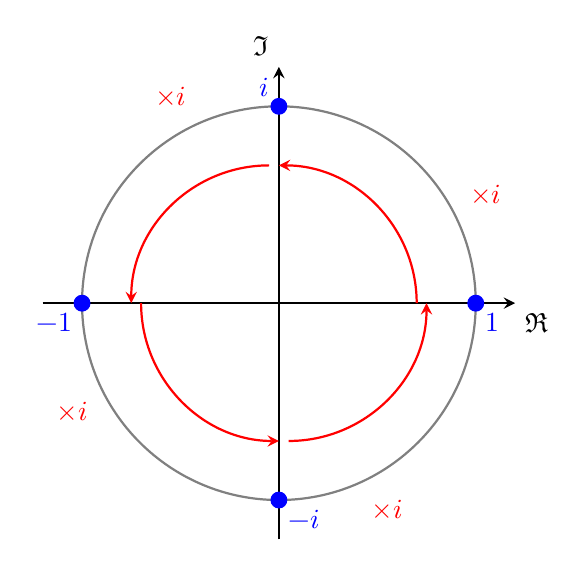
\begin{tikzpicture}[scale=2.5,>=stealth]
  % Unit circle
  \draw[gray, thick] (0,0) circle (1);
  % Axes
  \draw[->,thick] (-1.2,0) -- (1.2,0) node[below right] {$\Re$};
  \draw[->,thick] (0,-1.2) -- (0,1.2) node[above left] {$\Im$};
  % Points
  \filldraw[blue] (1,0) circle (0.04) node[below right] {$1$};
  \filldraw[blue] (0,1) circle (0.04) node[above left] {$i$};
  \filldraw[blue] (-1,0) circle (0.04) node[below left] {$-1$};
  \filldraw[blue] (0,-1) circle (0.04) node[below right] {$-i$};
  % Arrows for rotation with ×i labels outside the circle
  \draw[->, red, thick] (0.7,0) arc (0:90:0.7);
  \node[red] at (1.05,0.55) {$\times i$};  % label for 0->90
  \draw[->, red, thick] (-0.05,0.7) arc (90:180:0.7);
  \node[red] at (-0.55,1.05) {$\times i$};  % label for 90->180
  \draw[->, red, thick] (-0.7,0) arc (180:270:0.7);
  \node[red] at (-1.05,-0.55) {$\times i$}; % label for 180->270
  \draw[->, red, thick] (0.05,-0.7) arc (270:360:0.7);
  \node[red] at (0.55,-1.05) {$\times i$};  % label for 270->360
\end{tikzpicture}
\caption{Πολλαπλασιασμός με $i$: διαδοχικές περιστροφές κατά $90^\circ$ στον μοναδιαίο κύκλο.}
\label{fig:i_rotation}
\end{figure}

Αυτή η γεωμετρική ερμηνεία καθιστά τον τύπο Euler θεμελιώδη για την
περιγραφή ταλαντώσεων και κυμάτων: κάθε ημιτονοειδής ταλάντωση
\(A\cos(\omega t + \varphi)\) μπορεί να γραφεί ως το πραγματικό μέρος
μιας περιστρεφόμενης μιγαδικής ποσότητας
\(A e^{i(\omega t + \varphi)}\). Η περιστροφή αυτή αντιστοιχεί στη
μεταβολή της φάσης με τον χρόνο, και η προβολή στους άξονες δίνει τις
γνωστές τριγωνομετρικές συναρτήσεις.

\section{Σειρές Fourier}\label{ux3c3ux3b5ux3b9ux3c1ux3adux3c2-fourier}

Ο Joseph Fourier (1768--1830), εμπνευσμένος από το πρακτικό πρόβλημα της
διάδοσης της θερμότητας, ανέπτυξε μια μαθηματική θεωρία που αποδείχθηκε
επαναστατική. Το 1807 παρουσίασε στην Ακαδημία Επιστημών του Παρισιού
την εξίσωση θερμότητας και, για να τη λύσει, εισήγαγε τις σειρές
Fourier: την έκφραση μιας αυθαίρετης συνάρτησης ως αθροίσματος ημιτόνων
και συνημιτόνων. Αν και αρχικά αμφισβητήθηκε, το έργο του δημοσιεύτηκε
στο \emph{Théorie analytique de la chaleur} (Fourier 1822) και αποτελεί
σήμερα θεμέλιο της φασματικής ανάλυσης.

\subsection{Η εξίσωση
θερμότητας}\label{ux3b7-ux3b5ux3beux3afux3c3ux3c9ux3c3ux3b7-ux3b8ux3b5ux3c1ux3bcux3ccux3c4ux3b7ux3c4ux3b1ux3c2}

Θεωρούμε μια λεπτή μονωμένη ράβδο μήκους 1 m με τα άκρα της να
διατηρούνται σε σταθερή θερμοκρασία \(T(0,t)=T(1,t)=0\). Αν \(T(x,t)\)
είναι η θερμοκρασία στη θέση \(x\) τη στιγμή \(t\), η διάχυση της
θερμότητας περιγράφεται από την εξίσωση

\[
\frac{\partial T}{\partial t} = \alpha \frac{\partial^2 T}{\partial x^2},
\]

όπου \(\alpha\) είναι ο συντελεστής θερμικής διάχυσης. Ο ρυθμός
μεταβολής της θερμοκρασίας είναι ανάλογος της κυρτότητας της κατανομής
-- οι περιοχές με μεγάλη διαφορά θερμοκρασίας από τα γειτονικά σημεία
εξομαλύνονται ταχύτερα.

\subsection{Ανάλυση σε
ημίτονα}\label{ux3b1ux3bdux3acux3bbux3c5ux3c3ux3b7-ux3c3ux3b5-ux3b7ux3bcux3afux3c4ux3bfux3bdux3b1}

Ο Fourier παρατήρησε ότι αν η αρχική κατανομή \(T(x,0)\) αναπτυχθεί σε
σειρά ημιτόνων

\[
T(x,0) = \sum_{n=1}^{\infty} a_n \sin(n\pi x),
\]

τότε κάθε αρμονική εξελίσσεται ανεξάρτητα:

\[
T(x,t) = \sum_{n=1}^{\infty} a_n \, e^{-\alpha n^2 \pi^2 t} \sin(n\pi x).
\]

Οι υψηλές συχνότητες (μεγάλα \(n\)) αποσβένονται εκθετικά γρηγορότερα,
γι' αυτό η ράβδος εξομαλύνεται με τον χρόνο. Οι συντελεστές \(a_n\)
υπολογίζονται από την αρχική συνθήκη μέσω του τύπου

\[
a_n = 2\int_0^1 T(x,0)\,\sin(n\pi x)\,dx.
\]

Η ολοκλήρωση αυτή «μετράει» πόσο από κάθε συχνότητα περιέχεται στο σήμα
-- μια ιδέα που οδηγεί απευθείας στον μετασχηματισμό Fourier.

\section{Μετασχηματισμός
Fourier}\label{ux3bcux3b5ux3c4ux3b1ux3c3ux3c7ux3b7ux3bcux3b1ux3c4ux3b9ux3c3ux3bcux3ccux3c2-fourier}

Η έκφραση μιας συνάρτησης ως άθροισμα ημιτόνων και συνημιτόνων δεν
περιορίζεται στις λύσεις της εξίσωσης θερμότητας ούτε σε περιοδικά
σήματα. Ο μετασχηματισμός Fourier αποτελεί τη φυσική γενίκευση των
σειρών Fourier: ενώ η σειρά Fourier αναλύει περιοδικές συναρτήσεις σε
διακριτές αρμονικές, ο (συνεχής) Μετασχηματισμός Fourier αναλύει
μη-περιοδικά σήματα πεπερασμένης ενέργειας σε ένα συνεχές φάσμα
συχνοτήτων. Στην ψηφιακή πράξη, ωστόσο, τα δεδομένα μας είναι
δειγματοληπτημένα και πεπερασμένου μήκους. Γι' αυτό χρησιμοποιούμε τον
Διακριτό Μετασχηματισμό Fourier (DFT), ο οποίος αποτελεί την αντίστοιχη
έκδοση για ακολουθίες \(N\) σημείων και βασίζεται στον τύπο του Euler:
\(e^{i\theta} = \cos\theta + i\sin\theta\). Όπως θα δούμε, η μιγαδική
αυτή αναπαράσταση επιτρέπει την εναλλαγή μεταξύ του πεδίου του χρόνου (ή
του χώρου) και του πεδίου των συχνοτήτων -- εφαρμογή ζωτικής σημασίας σε
πολλούς τομείς, μεταξύ των οποίων η ανάλυση ηχητικών σημάτων και η
προσομοίωση κυμάτων στη θάλασσα.

\subsection{Από το σήμα στο φάσμα (Fourier
Transform)}\label{ux3b1ux3c0ux3cc-ux3c4ux3bf-ux3c3ux3aeux3bcux3b1-ux3c3ux3c4ux3bf-ux3c6ux3acux3c3ux3bcux3b1-fourier-transform}

Θέτοντας \(\theta = -\frac{2\pi kn}{N}\) στον τύπο του Euler,
\(e^{i\theta} = \cos\theta + i\sin\theta\), προκύπτει:

\[e^{-i\frac{2\pi kn}{N}} = \cos\!\left(\frac{2\pi kn}{N}\right) - i\sin\!\left(\frac{2\pi kn}{N}\right)\]

Ο διακριτός μετασχηματισμός Fourier (DFT) ορίζεται ως:

\[X_k = \sum_{n=0}^{N-1} x_n \, e^{-i\frac{2\pi kn}{N}}, \qquad k = 0,1,\dots,N-1\]

Αντικαθιστώντας την εκθετική με την τριγωνομετρική της μορφή:

\[X_k = \sum_{n=0}^{N-1} x_n \left[\cos\!\left(\frac{2\pi kn}{N}\right) - i\sin\!\left(\frac{2\pi kn}{N}\right)\right]\]

Επομένως, το πραγματικό και το φανταστικό μέρος του \(X_k\)
υπολογίζονται ξεχωριστά:

\[\begin{aligned}
\operatorname{Re}(X_k) &= \sum_{n=0}^{N-1} x_n \cos\!\left(\frac{2\pi kn}{N}\right), \\[4pt]
\operatorname{Im}(X_k) &= -\sum_{n=0}^{N-1} x_n \sin\!\left(\frac{2\pi kn}{N}\right).
\end{aligned}\]

\textbf{Γεωμετρική ερμηνεία:} Κάθε δείγμα \(x_n\) αντιστοιχεί σε ένα
διάνυσμα πάνω στον μοναδιαίο κύκλο με γωνία \(-\frac{2\pi kn}{N}\). Το
\(X_k\) είναι το διανυσματικό άθροισμα όλων των δειγμάτων, σταθμισμένων
με τα \(x_n\). Όταν η δοκιμαστική συχνότητα \(k\) ταιριάζει με κάποια
κυρίαρχη συχνότητα του σήματος, τα επιμέρους διανύσματα
προσανατολίζονται περίπου προς την ίδια κατεύθυνση, με αποτέλεσμα το
μέτρο \(|X_k|\) να γίνεται μεγάλο (εμφανίζεται κορυφή στο φάσμα).
Αντίθετα, όταν το \(k\) δεν αντιστοιχεί σε συχνότητα του σήματος, τα
διανύσματα κατανέμονται τυχαία γύρω από τον κύκλο και το άθροισμά τους
τείνει στο μηδέν.

\subsection{Από το φάσμα στο σήμα (Inverse Fourier
Transform)}\label{ux3b1ux3c0ux3cc-ux3c4ux3bf-ux3c6ux3acux3c3ux3bcux3b1-ux3c3ux3c4ux3bf-ux3c3ux3aeux3bcux3b1-inverse-fourier-transform}

Ο διακριτός μετασχηματισμός Fourier (DFT) μετέφερε ένα σήμα \(x_n\) από
το πεδίο του χρόνου στο πεδίο των συχνοτήτων \(X_k\). Η διαδικασία είναι
\textbf{αντιστρέψιμη}: από το φάσμα \(X_k\) μπορούμε να ανακτήσουμε το
αρχικό σήμα \(x_n\) μέσω του αντίστροφου μετασχηματισμού (IDFT), ο
οποίος ορίζεται ως:

\[
x_n = \frac{1}{N} \sum_{k=0}^{N-1} X_k \, e^{i\frac{2\pi kn}{N}}, \qquad n = 0,1,\dots,N-1.
\]

Η μορφή αυτή προκύπτει άμεσα από τον ορισμό του DFT: αν πολλαπλασιάσουμε
τον ορισμό του \(X_k\) με \(e^{i2\pi kn/N}\) και αθροίσουμε ως προς
\(k\), χρησιμοποιώντας την ταυτότητα ορθογωνιότητας

\[
\sum_{k=0}^{N-1} e^{i\frac{2\pi k(m-n)}{N}} = N \cdot \delta_{mn},
\]

παίρνουμε την αρχική ακολουθία \(x_n\).

\textbf{Γεωμετρική ερμηνεία:} Ο αντίστροφος μετασχηματισμός εκφράζει
κάθε δείγμα \(x_n\) ως σταθμισμένο άθροισμα περιστρεφόμενων φασόρων
\(e^{i2\pi kn/N}\), όπου το βάρος κάθε φάσορ είναι ακριβώς η φασματική
συνιστώσα \(X_k\). Με άλλα λόγια, το σήμα στο πεδίο του χρόνου
ανασυντίθεται από τις συχνότητες που το αποτελούν. Η ύπαρξη του
αντίστροφου μετασχηματισμού εγγυάται ότι καμία πληροφορία δεν χάνεται
κατά τη μετάβαση στο πεδίο των συχνοτήτων -- η αναπαράσταση είναι πλήρης
και αμφιμονοσήμαντη. Αυτή η ιδιότητα είναι θεμελιώδης σε όλες τις
εφαρμογές, από την επεξεργασία ήχου, όπου φιλτράρουμε στο φάσμα και
επαναφέρουμε στο χρόνο, μέχρι την προσομοίωση ωκεανού, όπου
κατασκευάζουμε το φάσμα και με IFFT (Inverse Fast Fourier Transform -
Αντίστροφος Γρήγορος Μετασχηματισμός Fourier) παίρνουμε την επιφάνεια.

Ο Μετασχηματισμός Fourier αποτελεί ένα ισχυρό εργαλείο για την ανάλυση
σημάτων σε συχνότητες -- είτε πρόκειται για ένα ηχητικό κύμα (1D) είτε
για μια επιφάνεια θάλασσας (2D). Η πρακτική του χρήση σε υπολογιστές
βασίζεται στον Γρήγορο Μετασχηματισμό Fourier (FFT) (Cooley and Tukey
1965), έναν αλγόριθμο που μειώνει την πολυπλοκότητα από \(O(N^2)\)
(απευθείας υπολογισμός του DFT) σε \(O(N \log N)\). Αυτή η επιτάχυνση
είναι που καθιστά εφικτή την προσομοίωση ωκεανού σε πραγματικό χρόνο,
ακόμα και με εκατομμύρια σημεία πλέγματος, ενώ παράλληλα επιτρέπει την
άμεση εφαρμογή της σε ήχο, εικόνα και τηλεπικοινωνίες.

\section{Πολυπλοκότητα}\label{ux3c0ux3bfux3bbux3c5ux3c0ux3bbux3bfux3baux3ccux3c4ux3b7ux3c4ux3b1}

Η παραπάνω διαφορά ανάγεται στο γεγονός ότι κάθε αλγόριθμος έχει ένα
εγγενές «κόστος» --- τον αριθμό των πράξεων που απαιτεί συναρτήσει του
μεγέθους \(n\) των δεδομένων εισόδου. Το κύριο εργαλείο για τη μελέτη
του είναι η Big‑O notation. Ένας αλγόριθμος με πολυπλοκότητα \(O(n^2)\)
σημαίνει ότι αν διπλασιαστούν τα δεδομένα, ο χρόνος εκτέλεσης
τετραπλασιάζεται, ενώ ένας \(O(n \log n)\) αλγόριθμος «αντέχει» σε πολύ
μεγαλύτερα δεδομένα, καθώς η αύξηση του κόστους είναι σχεδόν γραμμική. Η
διαφορά αυτή δεν είναι θεωρητική. Σε πραγματικά προβλήματα με
εκατομμύρια δεδομένα, η επιλογή αλγορίθμου καθορίζει αν μια εργασία
ολοκληρώνεται σε δευτερόλεπτα ή σε μέρες.

Για να γίνει αντιληπτό το μέγεθος, αρκεί να συγκρίνουμε τον 1D ήχο με τη
2D θάλασσα. Στον 1D ήχο, για ένα σήμα μήκους \(N\) δειγμάτων, ο
απευθείας DFT απαιτεί \(O(N^2)\) πράξεις. Για \(N=44100\) (π.χ. 1 sec CD
quality), αυτό αντιστοιχεί σε περίπου \(1.94\) δισεκατομμύρια πράξεις
--- ένα κόστος ήδη απαγορευτικό για επαναλαμβανόμενη επεξεργασία σε
πραγματικό χρόνο. Αντίθετα, σε μια προσομοίωση θάλασσας με πλέγμα
\(N \times N\) σημείων, ο 2D DFT χρειάζεται \(O(N^4)\) πράξεις συνολικά,
καθώς καθένα από τα \(N^2\) σημεία εξόδου απαιτεί άθροισμα πάνω σε όλα
τα \(N^2\) σημεία εισόδου. Το πρόβλημα δεν είναι απλώς το απόλυτο
μέγεθος, αλλά η αναλογία αύξησης: ο 1D DFT γίνεται 4 φορές πιο αργός
όταν διπλασιάζεται το \(N\), ενώ ο 2D DFT γίνεται 16 φορές πιο αργός ---
μια ραγδαία επιδείνωση που καθιστά τη ρεαλιστική θάλασσα υπολογιστικά
αδύνατη χωρίς εξειδικευμένους αλγορίθμους.

\subsection{Divide \& Conquer}\label{divide-conquer}

Η στρατηγική Divide \& Conquer είναι ένας από τους πιο ισχυρούς τρόπους
μείωσης της πολυπλοκότητας. Η λογική της είναι απλή: αντί να επιλύεις
ένα μεγάλο πρόβλημα απευθείας, το διασπάς αναδρομικά στη μέση, επιλύεις
κάθε τμήμα ανεξάρτητα και στη συνέχεια συνδυάζεις τα αποτελέσματα.

Ένα κλασικό παράδειγμα εφαρμογής της στρατηγικής αυτής αποτελεί η
ταξινόμηση. Η ταξινόμηση φυσαλίδας (bubble sort) συγκρίνει διαδοχικά
γειτονικά ζεύγη, ξεκινώντας από το τέλος του πίνακα και κινούμενη προς
την αρχή, μεταφέροντας το μικρότερο στοιχείο στη σωστή του θέση στην
αρχή του πίνακα. Χρειάζονται \(n-1\) διαβάσεις και σε κάθε διάβαση
γίνονται έως \(n-1\) συγκρίσεις, συνεπώς συνολικά περίπου \(n^2/2\)
πράξεις --- δηλαδή πολυπλοκότητα \(O(n^2)\) (Σχήμα
\ref{fig:bubblesort}). Αντίθετα, η ταξινόμηση με συγχώνευση (Merge Sort)
εφαρμόζει τη στρατηγική Divide \& Conquer: διασπά τον πίνακα στη μέση,
ταξινομεί αναδρομικά κάθε μισό και στη συνέχεια συγχωνεύει τα δύο
ταξινομημένα υποσύνολα. Το κόστος του μειώνεται σε \(O(n \log n)\), με
δραματικά αποτελέσματα σε μεγάλα σύνολα δεδομένων (Σχήμα
\ref{fig:mergesort}).

\begin{figure}[htbp]
\centering

% Ορισμός χρώματος για τους αριθμούς που συγκρίνονται
\definecolor{compcolor}{RGB}{255,140,0}
% Ορισμός χρώματος για αριθμούς ήδη ταξινομημένους
\definecolor{sortedcolor}{RGB}{10,255,10}

\begin{tikzpicture}[
    scale=0.8,
    transform shape,
    every node/.style={font=\small},
    basearr/.style={draw, inner sep=1pt, font=\ttfamily\small},
    bubblearr/.style={basearr, draw=splitcolor, fill=splitcolor!8, inner sep=1pt},
    bubblefinal/.style={basearr, draw=mergecolor, fill=mergecolor!15, inner sep=1pt, ultra thick},
    swap/.style={->, draw=swapcolor, thick, shorten >=1pt, shorten <=1pt},
    compare/.style={->, draw=gray!40, thick, shorten >=1pt, shorten <=1pt}
]

% ============================================================
% 1η ΔΙΑΒΑΣΗ
% ============================================================
\begin{scope}[xshift=-8cm]
\node[font=\bfseries, splitcolor] at (0, 11) {1η διάβαση};

\node[bubblearr] (start1) at (0, 10) {5·3·1·8·7·2·6·4};

\node[bubblearr] (s1a) at (0, 9) {5·3·1·8·7·2·\textcolor{compcolor}{6}·\textcolor{compcolor}{4}};
\draw[swap] (start1.south) -- (s1a.north);

\node[bubblearr] (s1b) at (0, 8) {5·3·1·8·7·\textcolor{compcolor}{2}·\textcolor{compcolor}{4}·6};
\draw[compare] (s1a.south) -- (s1b.north);

\node[bubblearr] (s1c) at (0, 7) {5·3·1·8·\textcolor{compcolor}{7}·\textcolor{compcolor}{2}·4·6};
\draw[swap] (s1b.south) -- (s1c.north);

\node[bubblearr] (s1d) at (0, 6) {5·3·1·\textcolor{compcolor}{8}·\textcolor{compcolor}{2}·7·4·6};
\draw[swap] (s1c.south) -- (s1d.north);

\node[bubblearr] (s1e) at (0, 5) {5·3·\textcolor{compcolor}{1}·\textcolor{compcolor}{2}·8·7·4·6};
\draw[compare] (s1d.south) -- (s1e.north);

\node[bubblearr] (s1f) at (0, 4) {5·\textcolor{compcolor}{3}·\textcolor{compcolor}{1}·2·8·7·4·6};
\draw[swap] (s1e.south) -- (s1f.north);

\node[bubblearr] (s1g) at (0, 3) {\textcolor{compcolor}{5}·\textcolor{compcolor}{1}·3·2·8·7·4·6};
\draw[swap] (s1f.south) -- (s1g.north);

\node[bubblefinal] (end1) at (0, 2) {\textcolor{sortedcolor}{1}·5·3·2·8·7·4·6};
\draw[swap] (s1g.south) -- (end1.north);
\end{scope}

% ============================================================
% 2η ΔΙΑΒΑΣΗ
% ============================================================
\begin{scope}[xshift=-3.2cm]
\node[font=\bfseries, splitcolor] at (0, 11) {2η διάβαση};

\node[bubblearr] (start2) at (0, 10) {\textcolor{sortedcolor}{1}·5·3·2·8·7·4·6};

\node[bubblearr] (s2a) at (0, 9) {\textcolor{sortedcolor}{1}·5·3·2·8·7·\textcolor{compcolor}{4}·\textcolor{compcolor}{6}};
\draw[compare] (start2.south) -- (s2a.north);

\node[bubblearr] (s2b) at (0, 8) {\textcolor{sortedcolor}{1}·5·3·2·8·\textcolor{compcolor}{7}·\textcolor{compcolor}{4}·6};
\draw[swap] (s2a.south) -- (s2b.north);

\node[bubblearr] (s2c) at (0, 7) {\textcolor{sortedcolor}{1}·5·3·2·\textcolor{compcolor}{8}·\textcolor{compcolor}{4}·7·6};
\draw[swap] (s2b.south) -- (s2c.north);

\node[bubblearr] (s2d) at (0, 6) {\textcolor{sortedcolor}{1}·5·3·\textcolor{compcolor}{2}·\textcolor{compcolor}{4}·8·7·6};
\draw[compare] (s2c.south) -- (s2d.north);

\node[bubblearr] (s2e) at (0, 5) {\textcolor{sortedcolor}{1}·5·\textcolor{compcolor}{3}·\textcolor{compcolor}{2}·4·8·7·6};
\draw[swap] (s2d.south) -- (s2e.north);

\node[bubblearr] (s2f) at (0, 4) {\textcolor{sortedcolor}{1}·\textcolor{compcolor}{5}·\textcolor{compcolor}{2}·3·4·8·7·6};
\draw[swap] (s2e.south) -- (s2f.north);

\node[bubblefinal] (end2) at (0, 3) {\textcolor{sortedcolor}{1}·\textcolor{sortedcolor}{2}·5·3·4·8·7·6};
\draw[compare] (s2f.south) -- (end2.north);
\end{scope}

% ============================================================
% 3η ΔΙΑΒΑΣΗ
% ============================================================
\begin{scope}[xshift=1.6cm]
\node[font=\bfseries, splitcolor] at (0, 11) {3η διάβαση};

\node[bubblearr] (start3) at (0, 10) {\textcolor{sortedcolor}{1}·\textcolor{sortedcolor}{2}·5·3·4·8·7·6};

\node[bubblearr] (s3a) at (0, 9) {\textcolor{sortedcolor}{1}·\textcolor{sortedcolor}{2}·5·3·4·8·\textcolor{compcolor}{6}·\textcolor{compcolor}{7}};
\draw[swap] (start3.south) -- (s3a.north);

\node[bubblearr] (s3b) at (0, 8) {\textcolor{sortedcolor}{1}·\textcolor{sortedcolor}{2}·5·3·4·\textcolor{compcolor}{6}·\textcolor{compcolor}{8}·7};
\draw[swap] (s3a.south) -- (s3b.north);

\node[bubblearr] (s3c) at (0, 7) {\textcolor{sortedcolor}{1}·\textcolor{sortedcolor}{2}·5·3·\textcolor{compcolor}{4}·\textcolor{compcolor}{6}·8·7};
\draw[compare] (s3b.south) -- (s3c.north);

\node[bubblearr] (s3d) at (0, 6) {\textcolor{sortedcolor}{1}·\textcolor{sortedcolor}{2}·3·\textcolor{compcolor}{5}·\textcolor{compcolor}{4}·6·8·7};
\draw[swap] (s3c.south) -- (s3d.north);

\node[bubblearr] (s3e) at (0, 5) {\textcolor{sortedcolor}{1}·\textcolor{sortedcolor}{2}·\textcolor{compcolor}{3}·\textcolor{compcolor}{5}·4·6·8·7};
\draw[swap] (s3d.south) -- (s3e.north);

\node[bubblefinal] (end3) at (0, 4) {\textcolor{sortedcolor}{1}·\textcolor{sortedcolor}{2}·\textcolor{sortedcolor}{3}·5·4·6·8·7};
\draw[compare] (s3e.south) -- (end3.north);
\end{scope}

% ============================================================
% 4η ΔΙΑΒΑΣΗ
% ============================================================
\begin{scope}[xshift=6.4cm]
\node[font=\bfseries, splitcolor] at (0, 11) {4η διάβαση};

\node[bubblearr] (start4) at (0, 10) {\textcolor{sortedcolor}{1}·\textcolor{sortedcolor}{2}·\textcolor{sortedcolor}{3}·5·4·6·8·7};

\node[bubblearr] (s4a) at (0, 9) {\textcolor{sortedcolor}{1}·\textcolor{sortedcolor}{2}·\textcolor{sortedcolor}{3}·5·4·6·\textcolor{compcolor}{7}·\textcolor{compcolor}{8}};
\draw[swap] (start4.south) -- (s4a.north);

\node[bubblearr] (s4b) at (0, 8) {\textcolor{sortedcolor}{1}·\textcolor{sortedcolor}{2}·\textcolor{sortedcolor}{3}·5·4·\textcolor{compcolor}{6}·\textcolor{compcolor}{7}·8};
\draw[compare] (s4a.south) -- (s4b.north);

\node[bubblearr] (s4c) at (0, 7) {\textcolor{sortedcolor}{1}·\textcolor{sortedcolor}{2}·\textcolor{sortedcolor}{3}·5·\textcolor{compcolor}{4}·\textcolor{compcolor}{6}·7·8};
\draw[compare] (s4b.south) -- (s4c.north);

\node[bubblearr] (s4d) at (0, 6) {\textcolor{sortedcolor}{1}·\textcolor{sortedcolor}{2}·\textcolor{sortedcolor}{3}·\textcolor{compcolor}{4}·\textcolor{compcolor}{5}·6·7·8};
\draw[swap] (s4c.south) -- (s4d.north);

\node[bubblefinal, very thick] (end4) at (0, 5) {\textcolor{sortedcolor}{1}·\textcolor{sortedcolor}{2}·\textcolor{sortedcolor}{3}·\textcolor{sortedcolor}{4}·5·6·7·8};
\draw[compare] (s4d.south) -- (end4.north);
\end{scope}

\end{tikzpicture}
\caption{Bubble Sort}
\label{fig:bubblesort}
\end{figure}

\begin{figure}[htbp]
\centering
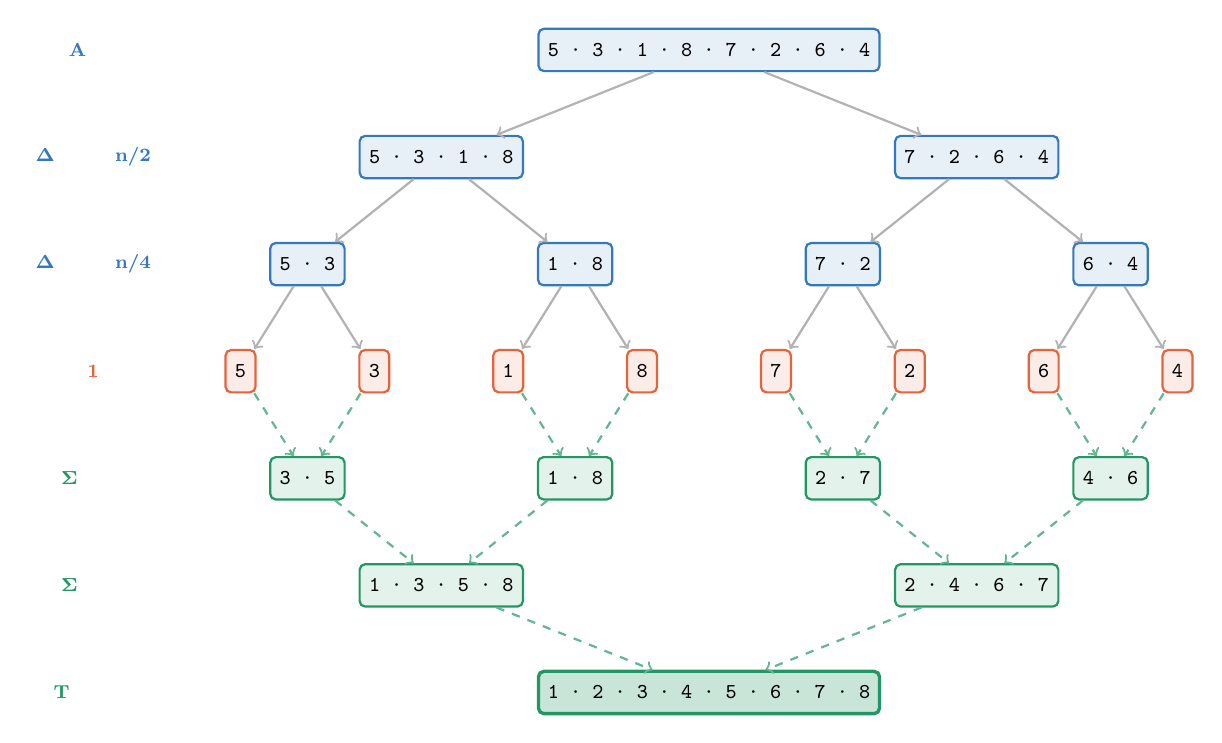
\begin{tikzpicture}[scale=0.85, transform shape, every node/.style={font=\small}]

% Level 0
\node[splitarr] (root) at (0, 0) {5 · 3 · 1 · 8 · 7 · 2 · 6 · 4};

% Level 1
\node[splitarr] (L1) at (-4, -1.6) {5 · 3 · 1 · 8};
\node[splitarr] (R1) at ( 4, -1.6) {7 · 2 · 6 · 4};

% Level 2
\node[splitarr] (LL2) at (-6, -3.2) {5 · 3};
\node[splitarr] (LR2) at (-2, -3.2) {1 · 8};
\node[splitarr] (RL2) at ( 2, -3.2) {7 · 2};
\node[splitarr] (RR2) at ( 6, -3.2) {6 · 4};

% Level 3 leaves
\node[leafarr] (a) at (-7,  -4.8) {5};
\node[leafarr] (b) at (-5,  -4.8) {3};
\node[leafarr] (c) at (-3,  -4.8) {1};
\node[leafarr] (d) at (-1,  -4.8) {8};
\node[leafarr] (e) at ( 1,  -4.8) {7};
\node[leafarr] (f) at ( 3,  -4.8) {2};
\node[leafarr] (g) at ( 5,  -4.8) {6};
\node[leafarr] (h) at ( 7,  -4.8) {4};

\draw[edge] (root)--(L1);
\draw[edge] (root)--(R1);
\draw[edge] (L1)--(LL2);
\draw[edge] (L1)--(LR2);
\draw[edge] (R1)--(RL2);
\draw[edge] (R1)--(RR2);
\draw[edge] (LL2)--(a);
\draw[edge] (LL2)--(b);
\draw[edge] (LR2)--(c);
\draw[edge] (LR2)--(d);
\draw[edge] (RL2)--(e);
\draw[edge] (RL2)--(f);
\draw[edge] (RR2)--(g);
\draw[edge] (RR2)--(h);

% Merge Level 2
\node[mergearr] (mLL) at (-6, -6.4) {3 · 5};
\node[mergearr] (mLR) at (-2, -6.4) {1 · 8};
\node[mergearr] (mRL) at ( 2, -6.4) {2 · 7};
\node[mergearr] (mRR) at ( 6, -6.4) {4 · 6};

% Merge Level 1
\node[mergearr] (mL) at (-4, -8.0) {1 · 3 · 5 · 8};
\node[mergearr] (mR) at ( 4, -8.0) {2 · 4 · 6 · 7};

% Merge Level 0
\node[mergearr, draw=mergecolor, fill=mergecolor!25, very thick]
(final) at (0, -9.6)
{1 · 2 · 3 · 4 · 5 · 6 · 7 · 8};

\draw[mergedge] (a)--(mLL);
\draw[mergedge] (b)--(mLL);
\draw[mergedge] (c)--(mLR);
\draw[mergedge] (d)--(mLR);
\draw[mergedge] (e)--(mRL);
\draw[mergedge] (f)--(mRL);
\draw[mergedge] (g)--(mRR);
\draw[mergedge] (h)--(mRR);
\draw[mergedge] (mLL)--(mL);
\draw[mergedge] (mLR)--(mL);
\draw[mergedge] (mRL)--(mR);
\draw[mergedge] (mRR)--(mR);
\draw[mergedge] (mL)--(final);
\draw[mergedge] (mR)--(final);

% Labels
\node[font=\footnotesize\bfseries, splitcolor] at (-9.2, 0.0) {Αρχικός};
\node[font=\footnotesize\bfseries, splitcolor] at (-9.2, -1.6) {Διαχωρισμός n/2};
\node[font=\footnotesize\bfseries, splitcolor] at (-9.2, -3.2) {Διαχωρισμός n/4};
\node[font=\footnotesize\bfseries, leafcolor] at (-9.2, -4.8) {1};
\node[font=\footnotesize\bfseries, mergecolor] at (-9.2, -6.4) {Συγχώνευση};
\node[font=\footnotesize\bfseries, mergecolor] at (-9.2, -8.0) {Συγχώνευση};
\node[font=\footnotesize\bfseries, mergecolor] at (-9.2, -9.6) {Ταξινομημένος};

\end{tikzpicture}
\caption{Merge Sort}
\label{fig:mergesort}
\end{figure}

Αυτή ακριβώς την αρχή εφάρμοσαν οι Cooley \& Tukey (Cooley and Tukey
1965) στον υπολογισμό του μετασχηματισμού Fourier: ενώ ο απευθείας
υπολογισμός (DFT) απαιτεί \(O(n^2)\) πράξεις, ο γρήγορος μετασχηματισμός
Fourier (FFT) διασπά αναδρομικά το πρόβλημα και το ανάγει σε
\(O(n \log n)\), καθιστώντας υπολογιστικά εφικτό ό,τι ήταν ως τότε
απαγορευτικό.

Στην περίπτωση της 2D θάλασσας, ο 2D FFT μειώνει το συνολικό κόστος από
\(O(N^4)\) σε \(O(N^2 \log N)\). Για \(N=512\), αυτό σημαίνει ότι οι
\(68 \times 10^9\) πράξεις του απευθείας DFT μετατρέπονται σε περίπου
\(512^2 \cdot \log_2(512) = 262144 \cdot 9 \approx 2.36\) εκατομμύρια
πράξεις --- μια μείωση της τάξης των 30.000 φορών. Αυτή ακριβώς η
επιτάχυνση είναι που επιτρέπει την προσομοίωση ρεαλιστικών ωκεάνιων
επιφανειών σε πραγματικό χρόνο μέσα σε βιντεοπαιχνίδια και ταινίες.

\section{Fast Fourier Transform}\label{fast-fourier-transform}

Ο FFT βασίζεται στην ίδια λογική Divide \& Conquer που περιγράφηκε στο
Merge Sort: επιταχύνει τον DFT από \(O(N^2)\) σε \(O(N \log N)\) μέσω
μιας αναδρομικής διάσπασης που αξιοποιεί συμμετρίες. Η διάσπαση αυτή
βασίζεται σε τρεις έννοιες: τα πολυώνυμα, τις \(N\)-οστές ρίζες της
μονάδας και τον διαχωρισμό άρτιων και περιττών όρων.

\subsection{Πολυώνυμα (αναπαράσταση
συντελεστών)}\label{ux3c0ux3bfux3bbux3c5ux3ceux3bdux3c5ux3bcux3b1-ux3b1ux3bdux3b1ux3c0ux3b1ux3c1ux3acux3c3ux3c4ux3b1ux3c3ux3b7-ux3c3ux3c5ux3bdux3c4ux3b5ux3bbux3b5ux3c3ux3c4ux3ceux3bd}

Ένα πολυώνυμο βαθμού \(n-1\) γράφεται ως
\(A(x) = a_0 + a_1 x + a_2 x^2 + \cdots + a_{n-1} x^{n-1}\) ή ισοδύναμα
ως διάνυσμα συντελεστών \((a_0, a_1, \ldots, a_{n-1})\). Για την
αποτελεσματική υλοποίηση του FFT, μας ενδιαφέρουν τρεις βασικές πράξεις
σε πολυώνυμα: η πρόσθεση, ο πολλαπλασιασμός και η αποτίμηση (υπολογισμός
τιμής για δοσμένο \(x_0\)). Ο πίνακας που ακολουθεί συνοψίζει τις
πολυπλοκότητές τους:

\begin{longtable}[]{@{}lll@{}}
\toprule\noalign{}
Πράξη & Τύπος & Πολυπλοκότητα \\
\midrule\noalign{}
\endhead
\bottomrule\noalign{}
\endlastfoot
Αποτίμηση (Horner) & \(A(x_0)\) & \(O(n)\) \\
Πρόσθεση & \(C(x) = A(x) + B(x)\) & \(O(n)\) \\
Πολλαπλασιασμός & \(C(x) = A(x) \cdot B(x)\) & \(O(n^2)\) \\
\end{longtable}

Η απλοϊκή μέθοδος πολλαπλασιασμού πολυωνύμων βαθμού \(n-1\) απαιτεί
\(n^2\) πολλαπλασιασμούς, επειδή κάθε συντελεστής του \(A(x)\)
πολλαπλασιάζεται με κάθε συντελεστή του \(B(x)\). Η πρόσθεση είναι απλή,
απλά προστίθενται οι συντελεστές ίδιας δύναμης. Για την αποτίμηση, το
σχήμα του Horner μετασχηματίζει το πολυώνυμο στη μορφή
\(A(x) = a_0 + x\bigl(a_1 + x(a_2 + \cdots + x(a_{n-2} + x\,a_{n-1})\cdots)\bigr)\).
Ξεκινώντας από τον υψηλότερο συντελεστή \(a_{n-1}\) και προχωρώντας προς
τα κάτω, κάθε βήμα απαιτεί μία πρόσθεση και έναν πολλαπλασιασμό.
Επομένως, με \(n\) βήματα, το συνολικό κόστος είναι \(O(n)\) --- αντί
για \(O(n^2)\) αν υπολογίζαμε κάθε δύναμη \(x^k\) χωριστά. Αυτή η
γραμμική πολυπλοκότητα είναι κρίσιμη για την αποδοτικότητα του FFT.

\subsection{Πολυώνυμα (αναπαράσταση
σημείων)}\label{ux3c0ux3bfux3bbux3c5ux3ceux3bdux3c5ux3bcux3b1-ux3b1ux3bdux3b1ux3c0ux3b1ux3c1ux3acux3c3ux3c4ux3b1ux3c3ux3b7-ux3c3ux3b7ux3bcux3b5ux3afux3c9ux3bd}

Μια επιπλέον ιδιότητα, θεμελιώδης για τον FFT, είναι ότι κάθε πολυώνυμο
βαθμού \(d\) μπορεί να αναπαρασταθεί μοναδικά από \(d+1\) σημεία
\((x_i, A(x_i))\), αρκεί τα \(x_i\) να είναι διακριτά. Η μετάβαση από τα
σημεία στους συντελεστές γίνεται μέσω της παρεμβολής Lagrange:

\[
A(x) = \sum_{i=0}^{d} y_i \cdot L_i(x), \qquad
L_i(x) = \prod_{\substack{0 \le j \le d \\ j \ne i}} \frac{x - x_j}{x_i - x_j},
\]

όπου \(y_i = A(x_i)\). Οι πολυωνυμικές συναρτήσεις \(L_i(x)\)
εξασφαλίζουν ότι \(L_i(x_i)=1\) και \(L_i(x_j)=0\) για \(j \ne i\),
οπότε το άθροισμα «περνά» ακριβώς από τα σημεία \((x_i, y_i)\).

Η αναπαράσταση σημείων είναι χρήσιμη επειδή αλλάζει την πολυπλοκότητα
βασικών πράξεων:

\begin{longtable}[]{@{}lll@{}}
\toprule\noalign{}
Πράξη & Τύπος & Πολυπλοκότητα \\
\midrule\noalign{}
\endhead
\bottomrule\noalign{}
\endlastfoot
Αποτίμηση (Lagrange) & \(A(x_0)\) & \(O(n^2)\) \\
Πρόσθεση & \(C(x_i) = A(x_i) + B(x_i)\) & \(O(n)\) \\
Πολλαπλασιασμός & \(C(x_i) = A(x_i) \cdot B(x_i)\) & \(O(n)\) \\
\end{longtable}

Στον πολλαπλασιασμό, αν έχουμε δύο πολυώνυμα αναπαραστημένα στα ίδια
σημεία \(x_i\), το γινόμενό τους προκύπτει απλά ως
\(C(x_i) = A(x_i) \cdot B(x_i)\), με κόστος \(O(n)\). Αντίθετα, στην
αναπαράσταση συντελεστών ο πολλαπλασιασμός κοστίζει \(O(n^2)\). Αυτό
οδηγεί στη στρατηγική:

\begin{enumerate}
\def\labelenumi{\arabic{enumi}.}
\item
  Μετατρέπουμε \(A\) και \(B\) από συντελεστές σε σημεία (αποτίμηση).
\item
  Πολλαπλασιάζουμε σημείο-προς-σημείο (κόστος \(O(n)\)).
\item
  Μετατρέπουμε το αποτέλεσμα από σημεία πίσω σε συντελεστές (παρεμβολή).
\end{enumerate}

Το συνολικό κόστος καθορίζεται από την αποτίμηση και την παρεμβολή. Αν
επιλέξουμε τυχαία σημεία \(x_i\), και οι δύο αυτές διαδικασίες κοστίζουν
\(O(n^2)\), οπότε το κέρδος μηδενίζεται. Χρειαζόμαστε επομένως ένα
σύνολο \(n\) σημείων για το οποίο η αποτίμηση και η παρεμβολή μπορούν να
γίνουν σε \(O(n \log n)\). Αυτό το σύνολο είναι οι \(n\)-οστές ρίζες της
μονάδας στο μιγαδικό επίπεδο. Η συμμετρία τους επιτρέπει την αναδρομική
διάσπαση του προβλήματος σε μικρότερα ίδιας μορφής, μειώνοντας δραστικά
το κόστος --- ακριβώς τη λογική που εκμεταλλεύεται ο FFT.

\subsection{n-οστές ρίζες της
μονάδας}\label{n-ux3bfux3c3ux3c4ux3adux3c2-ux3c1ux3afux3b6ux3b5ux3c2-ux3c4ux3b7ux3c2-ux3bcux3bfux3bdux3acux3b4ux3b1ux3c2}

Οι n-οστές ρίζες της μονάδας είναι οι μιγαδικοί αριθμοί \(z\) που
ικανοποιούν την εξίσωση \(z^n = 1\), ή ισοδύναμα \(z^n - 1 = 0\). Στο
μιγαδικό επίπεδο, οι λύσεις βρίσκονται πάνω στον μοναδιαίο κύκλο και
σχηματίζουν κανονικό \(n\)-γωνο. Η θεμελιώδης ρίζα είναι

\[
\omega_N = e^{2\pi i / N} = \cos\left(\frac{2\pi}{N}\right) + i \sin\left(\frac{2\pi}{N}\right),
\]

και όλες οι ρίζες είναι οι δυνάμεις \(\omega_N^k\) για
\(k = 0,1,\dots,N-1\). Οι βασικές τους ιδιότητες είναι:

\begin{itemize}
\tightlist
\item
  Κυκλικότητα: \(\omega_N^{k+N} = \omega_N^k\) (περιοδικότητα με περίοδο
  \(N\)).
\item
  Συμμετρία: \(\omega_N^{k+N/2} = -\omega_N^k\) (ισχύει όταν \(N\)
  άρτιος).
\item
  Αναγωγή: \((\omega_N^k)^2 = \omega_{N/2}^k\) (για άρτιο \(N\), τα
  τετράγωνα μεταβαίνουν σε ρίζες τάξης \(N/2\)).
\end{itemize}

Το Σχήμα \ref{fig:roots_of_unity} δείχνει την περίπτωση \(N=8\): οι
ρίζες σχηματίζουν κανονικό οκτάγωνο, η θεμελιώδης γωνία \(2\pi/N\)
φαίνεται με μπλε τόξο, και το αντιδιαμετρικό ζεύγος
\(\omega_8^1,\omega_8^5\) απεικονίζει με κόκκινο ακριβώς τη συμμετρία
\(\omega_N^{k+N/2}=-\omega_N^k\). Αυτές οι συμμετρίες αποτελούν την
κρυφή δομή που επιτρέπει την επιτάχυνση του μετασχηματισμού Fourier
(Cooley and Tukey 1965).

\begin{figure}[htbp]
\centering
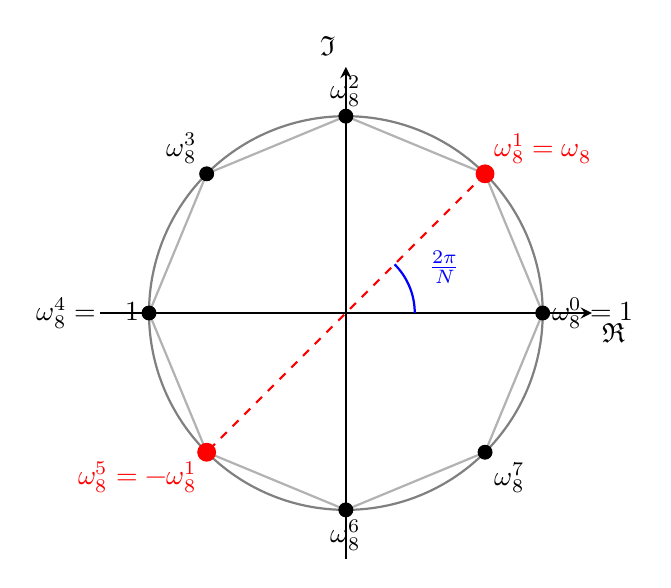
\begin{tikzpicture}[scale=2.5,>=stealth]
  % Unit circle
  \draw[gray, thick] (0,0) circle (1);
  % Axes
  \draw[->,thick] (-1.25,0) -- (1.25,0) node[below right] {$\Re$};
  \draw[->,thick] (0,-1.25) -- (0,1.25) node[above left] {$\Im$};

  % Regular octagon connecting the 8th roots of unity
  \draw[gray!60, thick]
    (0:1) -- (45:1) -- (90:1) -- (135:1) -- (180:1)
    -- (225:1) -- (270:1) -- (315:1) -- cycle;

  % The 8 roots, plain black dots + labels
  \filldraw[black] (0:1) circle (0.035) node[right] {$\omega_8^0=1$};
  \filldraw[black] (90:1) circle (0.035) node[above] {$\omega_8^2$};
  \filldraw[black] (135:1) circle (0.035) node[above left] {$\omega_8^3$};
  \filldraw[black] (180:1) circle (0.035) node[left] {$\omega_8^4=-1$};
  \filldraw[black] (270:1) circle (0.035) node[below] {$\omega_8^6$};
  \filldraw[black] (315:1) circle (0.035) node[below right] {$\omega_8^7$};

  % Antipodal (symmetric) pair k=1 and k=5, highlighted in red
  \draw[red, dashed, thick] (45:1) -- (225:1);
  \filldraw[red] (45:1) circle (0.045) node[above right] {$\omega_8^1=\omega_8$};
  \filldraw[red] (225:1) circle (0.045) node[below left] {$\omega_8^5=-\omega_8^1$};

  % Angle arc showing the fundamental step 2*pi/N between omega^0 and omega^1
  \draw[blue, thick] (0.35,0) arc (0:45:0.35);
  \node[blue] at (25:0.55) {$\frac{2\pi}{N}$};

\end{tikzpicture}
\caption{Οι $8$-οστές ρίζες της μονάδας στο μιγαδικό επίπεδο ($N=8$).}
\label{fig:roots_of_unity}
\end{figure}

\subsection{Διαχωρισμός άρτιων/περιττών όρων
(Cooley)}\label{ux3b4ux3b9ux3b1ux3c7ux3c9ux3c1ux3b9ux3c3ux3bcux3ccux3c2-ux3acux3c1ux3c4ux3b9ux3c9ux3bdux3c0ux3b5ux3c1ux3b9ux3c4ux3c4ux3ceux3bd-ux3ccux3c1ux3c9ux3bd-cooley}

Η βασική παρατήρηση των Cooley \& Tukey (Cooley and Tukey 1965) είναι
ότι ο διακριτός μετασχηματισμός Fourier (DFT) ενός σήματος μήκους \(N\)
(άρτιου) μπορεί να εκφραστεί ως συνδυασμός δύο DFT μήκους \(N/2\) ---
έναν για τους άρτιους δείκτες και έναν για τους περιττούς.

Έστω \(\mathbf{a} = (a_0, a_1, \dots, a_{N-1})\). Χωρίζουμε σε άρτιους
\(a_0, a_2, a_4, \dots\) και περιττούς όρους \(a_1, a_3, a_5, \dots\) οι
οποίοι ορίζουν τα πολυώνυμα:

\begin{itemize}
\tightlist
\item
  \(A_{\text{even}}(x) = \sum_{k=0}^{N/2-1} a_{2k} x^k = (a_0, a_2, a_4, \ldots)\)
\item
  \(A_{\text{odd}}(x) = \sum_{k=0}^{N/2-1} a_{2k+1} x^k = (a_1, a_3, a_5, \ldots)\)
\end{itemize}

Τότε ο DFT στο σημείο \(\omega_N^{-k}\) γράφεται:

\[
A(\omega_N^{-k}) = A_{\text{even}}(\omega_{N/2}^{-k}) \;+\; \omega_N^{-k} \cdot A_{\text{odd}}(\omega_{N/2}^{-k}).
\]

Ο δείκτης \(k\) λαμβάνει τιμές \(0, 1, \ldots, N-1\). Για \(k < N/2\), η
παραπάνω σχέση δίνει απευθείας το αποτέλεσμα. Για \(k \ge N/2\), η σχέση
εξακολουθεί να ισχύει, αλλά τα \(A_{\text{even}}(\omega_{N/2}^{-k})\)
και \(A_{\text{odd}}(\omega_{N/2}^{-k})\) επαναχρησιμοποιούν τις τιμές
για \(k - N/2\), λόγω της περιοδικότητας της εκθετικής συνάρτησης. Αντί
να υπολογίζουμε \(N\) τιμές απευθείας (κόστος \(O(N^2)\)), υπολογίζουμε
δύο μικρότερα DFT μεγέθους \(N/2\) το καθένα. Αυτή η αναδρομική διάσπαση
αποτελεί υλοποίηση της στρατηγικής Divide \& Conquer που περιγράφηκε
νωρίτερα.

\subsection{Cooley-Tukey FFT
βήμα-βήμα}\label{cooley-tukey-fft-ux3b2ux3aeux3bcux3b1-ux3b2ux3aeux3bcux3b1}

Η παραπάνω διάσπαση εφαρμόζεται αναδρομικά ως εξής.

\textbf{Βήμα 1 (Διαίρεση):}\\
Για \(N = 2^m\) (δύναμη του 2), το αρχικό διάνυσμα διαχωρίζεται σε άρτια
και περιττά στοιχεία. Στη συνέχεια, η ίδια διαδικασία εφαρμόζεται σε
κάθε υποδιάνυσμα μήκους \(N/2\), και επαναλαμβάνεται έως ότου προκύψουν
διανύσματα μήκους 1, όπου ο DFT είναι τετριμμένος.

\textbf{Βήμα 2 (Σύνθεση):}\\
Για κάθε \(k = 0, 1, \dots, N/2 - 1\), ο βασικός υπολογισμός για το
ζεύγος των δεικτών \(k\) και \(k+N/2\) ονομάζεται \textbf{πεταλούδα
(butterfly)} και δίνεται από τις σχέσεις:

\[
\begin{aligned}
A(\omega_N^{-k}) &= A_{\text{even}}(\omega_{N/2}^{-k}) + \omega_N^{-k} \cdot A_{\text{odd}}(\omega_{N/2}^{-k}) \\
A(\omega_N^{-(k+N/2)}) &= A_{\text{even}}(\omega_{N/2}^{-k}) - \omega_N^{-k} \cdot A_{\text{odd}}(\omega_{N/2}^{-k})
\end{aligned}
\]

(Η δεύτερη σχέση προκύπτει από τη συμμετρία
\(\omega_N^{-(k+N/2)} = -\omega_N^{-k}\).)

\textbf{Βήμα 3 (Επίπεδα και συνολικό κόστος):}\\
Η αναδρομή δημιουργεί \(\log_2 N\) επίπεδα. Σε κάθε επίπεδο εκτελούνται
\(N/2\) πεταλούδες (μία για κάθε ζεύγος), και κάθε πεταλούδα απαιτεί
σταθερό αριθμό πράξεων. Επομένως, το συνολικό κόστος είναι:

\[
T(N) = O(N \log N).
\]

\textbf{Παράδειγμα για \(N=4\):}\\
- Επίπεδο 0: είσοδος \((a_0,a_1,a_2,a_3)\)\\
- Διαίρεση σε άρτια \((a_0,a_2)\) και περιττά \((a_1,a_3)\)\\
- Υπολογισμός DFT μήκους 2 (2 πεταλούδες)\\
- Σύνθεση με 2 πεταλούδες για το μήκος 4

Το Σχήμα \ref{fig:fft_butterfly_n4} δείχνει το πλήρες διάγραμμα ροής: η
είσοδος \((a_0,a_2,a_1,a_3)\) εμφανίζεται σε bit-reversed σειρά, το
πρώτο στάδιο υπολογίζει δύο τετριμμένα DFT μήκους 2 (συντελεστής
\(\omega_2^0=1\), απλή πρόσθεση/αφαίρεση), και το δεύτερο στάδιο
συνδυάζει τα ενδιάμεσα \(b_i\) με τους πραγματικούς συντελεστές
\(\omega_4^{-k}\), δίνοντας τελικά \(A(\omega_4^{-k})\) στη φυσική σειρά
\(k=0,1,2,3\).

\begin{figure}[htbp]
\centering
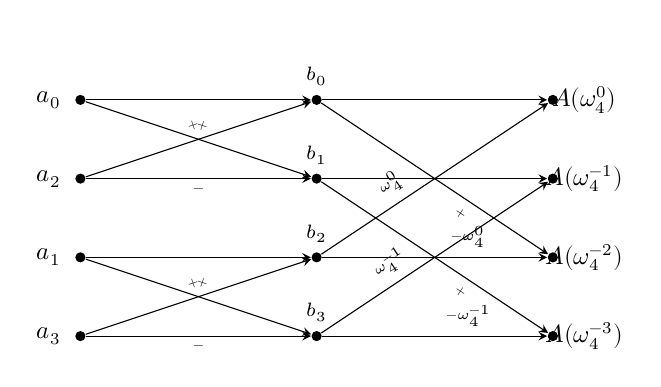
\begin{tikzpicture}[scale=1, >=stealth, every node/.style={font=\small}]

  % --- Οριζόντιες θέσεις σταδίων ---
  \def\xin{0}
  \def\xmid{3}
  \def\xout{6}

  % --- Κατακόρυφες θέσεις (4 γραμμές) ---
  \def\ya{3}
  \def\yb{2}
  \def\yc{1}
  \def\yd{0}

  % ============================================================
  % Είσοδοι (bit-reversed σειρά: a0, a2, a1, a3)
  % ============================================================
  \node[circle, fill=black, inner sep=1.3pt] (in0) at (\xin,\ya) { };
  \node at (-0.4,\ya) {$a_0$};
  \node[circle, fill=black, inner sep=1.3pt] (in1) at (\xin,\yb) { };
  \node at (-0.4,\yb) {$a_2$};
  \node[circle, fill=black, inner sep=1.3pt] (in2) at (\xin,\yc) { };
  \node at (-0.4,\yc) {$a_1$};
  \node[circle, fill=black, inner sep=1.3pt] (in3) at (\xin,\yd) { };
  \node at (-0.4,\yd) {$a_3$};

  % ============================================================
  % Στάδιο 1: δύο πεταλούδες μήκους 2 (τετριμμένος συντελεστής ω_2^0=1)
  % ============================================================
  \node[circle, fill=black, inner sep=1.3pt] (m0) at (\xmid,\ya) { };
  \node[circle, fill=black, inner sep=1.3pt] (m1) at (\xmid,\yb) { };
  \node[circle, fill=black, inner sep=1.3pt] (m2) at (\xmid,\yc) { };
  \node[circle, fill=black, inner sep=1.3pt] (m3) at (\xmid,\yd) { };

  % Πεταλούδα 1: (a0,a2) -> (b0,b1)
  \draw[->] (in0) -- (m0);
  \draw[->] (in0) -- (m1) node[midway, above, sloped, font=\tiny] {$+$};
  \draw[->] (in1) -- (m0) node[midway, above, sloped, font=\tiny] {$+$};
  \draw[->] (in1) -- (m1) node[midway, below, sloped, font=\tiny] {$-$};

  % Πεταλούδα 2: (a1,a3) -> (b2,b3)
  \draw[->] (in2) -- (m2);
  \draw[->] (in2) -- (m3) node[midway, above, sloped, font=\tiny] {$+$};
  \draw[->] (in3) -- (m2) node[midway, above, sloped, font=\tiny] {$+$};
  \draw[->] (in3) -- (m3) node[midway, below, sloped, font=\tiny] {$-$};

  \node at (\xmid,3.3) {\scriptsize $b_0$};
  \node at (\xmid,2.3) {\scriptsize $b_1$};
  \node at (\xmid,1.3) {\scriptsize $b_2$};
  \node at (\xmid,0.3) {\scriptsize $b_3$};

  % ============================================================
  % Στάδιο 2: πεταλούδες μήκους 4 (με πραγματικούς συντελεστές ω_4^{-k})
  % ============================================================
  \node[circle, fill=black, inner sep=1.3pt] (out0) at (\xout,\ya) { };
  \node[circle, fill=black, inner sep=1.3pt] (out1) at (\xout,\yb) { };
  \node[circle, fill=black, inner sep=1.3pt] (out2) at (\xout,\yc) { };
  \node[circle, fill=black, inner sep=1.3pt] (out3) at (\xout,\yd) { };

  % Πεταλούδα 3: (b0,b2) -> (A0,A2), συντελεστής ω_4^0=1
  \draw[->] (m0) -- (out0);
  \draw[->] (m0) -- (out2) node[pos=0.65, below, sloped, font=\tiny] {$+$};
  \draw[->] (m2) -- (out0) node[pos=0.35, above, sloped, font=\tiny] {$\omega_4^{0}$};
  \draw[->] (m2) -- (out2) node[pos=0.65, above, sloped, font=\tiny] {$-\omega_4^{0}$};

  % Πεταλούδα 4: (b1,b3) -> (A1,A3), συντελεστής ω_4^{-1}
  \draw[->] (m1) -- (out1);
  \draw[->] (m1) -- (out3) node[pos=0.65, below, sloped, font=\tiny] {$+$};
  \draw[->] (m3) -- (out1) node[pos=0.35, above, sloped, font=\tiny] {$\omega_4^{-1}$};
  \draw[->] (m3) -- (out3) node[pos=0.65, above, sloped, font=\tiny] {$-\omega_4^{-1}$};

  \node at (6.4,\ya) {$A(\omega_4^{0})$};
  \node at (6.4,\yb) {$A(\omega_4^{-1})$};
  \node at (6.4,\yc) {$A(\omega_4^{-2})$};
  \node at (6.4,\yd) {$A(\omega_4^{-3})$};

  % --- Ετικέτες σταδίων ---
  \node[font=\footnotesize\bfseries] at (\xin, 3.8) {};
  \node[font=\footnotesize\bfseries] at (\xmid, 3.8) {};
  \node[font=\footnotesize\bfseries] at (\xout, 3.8) {};

\end{tikzpicture}
\caption{Διάγραμμα πεταλούδας του FFT για $N=4$.}
\label{fig:fft_butterfly_n4}
\end{figure}

Σύνολο πράξεων: ο FFT απαιτεί \(\frac{N}{2} \log_2 N = 2 \cdot 2 = 4\)
πεταλούδες (μία πράξη πολλαπλασιασμού μιγαδικών ανά πεταλούδα), ενώ ο
απευθείας DFT απαιτεί \(N^2 = 16\) πολλαπλασιασμούς μιγαδικών. Για
μεγάλα \(N\), η διαφορά γίνεται τεράστια.

Αυτή ακριβώς η τεχνική -- η αναδρομική διάσπαση σε άρτιους και περιττούς
όρους και η επανασύνθεση με πεταλούδες -- αποτελεί τον Γρήγορο
Μετασχηματισμό Fourier (FFT). Χάρη σε αυτήν, η ανάλυση ήχου, η
επεξεργασία εικόνας (π.χ. συμπίεση JPEG, φιλτράρισμα), αλλά και η
προσομοίωση της θάλασσας έγιναν υπολογιστικά εφικτές.

\section{Θάλασσα}\label{ux3b8ux3acux3bbux3b1ux3c3ux3c3ux3b1}

Η προσομοίωση μιας ρεαλιστικής θάλασσας συναντά ένα θεμελιώδες
υπολογιστικό εμπόδιο: η πλήρης επίλυση των εξισώσεων Navier--Stokes
(Navier 1822; Stokes 1845) παρουσιάζει απαγορευτική υπολογιστική
πολυπλοκότητα -- ακόμα και για μικρό όγκο νερού απαιτούνται
υπερυπολογιστές, πόσο μάλλον για ανοιχτή θάλασσα. Η βιομηχανία βρήκε τη
λύση στην εργασία του Jerry Tessendorf (Tessendorf 2001), ο οποίος
πρότεινε την προσομοίωση όχι του ίδιου του νερού, αλλά των συχνοτήτων
των κυμάτων του. Αντί για δισεκατομμύρια μόρια, αρκούν λίγα ημίτονα και
συνημίτονα --- ακριβώς τις συναρτήσεις που, όπως είδαμε, οι υπολογιστές
μπορούν να προσεγγίσουν αποτελεσματικά μέσω πολυωνύμων Taylor (μια
προσέγγιση που αξιοποίησε ο Euler για να συνδέσει τις εκθετικές με τις
τριγωνομετρικές συναρτήσεις). Η σύνθεση πολλών συχνοτήτων γίνεται με τον
μετασχηματισμό Fourier, και χάρη στον γρήγορο αλγόριθμο FFT, το
λογισμικό μπορεί να υπολογίζει την επιφάνεια της θάλασσας σε κλάσματα
του δευτερολέπτου. Έτσι, πίσω από κάθε ψηφιακό ωκεανό σε ταινία ή
βιντεοπαιχνίδι, κρύβεται η ίδια μαθηματική ιδέα: ανάλυση της
πολυπλοκότητας σε απλές αρμονικές συχνότητες, βασιζόμενη στους Taylor,
Euler και Fourier.

Η ψηφιακή θάλασσα κατασκευάζεται στο πεδίο συχνοτήτων και μεταφράζεται
στον φυσικό χώρο μέσω αντίστροφου μετασχηματισμού Fourier. Αντί να
οριστεί κάθε κύμα χειροκίνητα, ορίζεται το φάσμα ενέργειας και ο
μετασχηματισμός κατασκευάζει την επιφάνεια.

\subsection{Κυματαριθμοί (Wave
Vectors)}\label{ux3baux3c5ux3bcux3b1ux3c4ux3b1ux3c1ux3b9ux3b8ux3bcux3bfux3af-wave-vectors}

Η προσομοίωση της θάλασσας δεν ξεκινά απευθείας από τη γεωμετρία της
επιφάνειας, αλλά από το πεδίο συχνοτήτων (frequency domain). Αντί δηλαδή
να αποθηκεύουμε το ύψος κάθε σημείου του ωκεανού, περιγράφουμε τη
θάλασσα ως άθροισμα πολλών απλών κυμάτων διαφορετικών μηκών και
κατευθύνσεων. Για τον σκοπό αυτό ορίζεται ένα πλέγμα \(N \times N\) στο
πεδίο των συχνοτήτων. Κάθε κελί \((i,j)\) του πλέγματος αντιστοιχεί σε
μία πιθανή κυματική συνιστώσα, δηλαδή σε ένα επίπεδο κύμα που μπορεί να
συμμετέχει στη σύνθεση της τελικής επιφάνειας. Σε κάθε κελί
αντιστοιχίζεται ένας κυματαριθμός \(\vec{k} = (k_x, k_z)\) όπου:

\[
k_x = \frac{2\pi}{L}i,
\qquad
k_z = \frac{2\pi}{L}j
\]

και \(L\) είναι το φυσικό μέγεθος της προσομοιούμενης περιοχής σε μέτρα,
ενώ \(i,j \in \{-N/2,\dots,N/2-1\}\).

Ο κυματαριθμός \(\vec{k}\) καθορίζει τόσο την κατεύθυνση διάδοσης όσο
και το μήκος κύματος. Το μέτρο του δίνεται από τη σχέση
\(k = |\vec{k}| = \sqrt{k_x^2 + k_z^2}\) και συνδέεται με το μήκος
κύματος μέσω της σχέσης \(\lambda = \frac{2\pi}{k}\). Μικρές τιμές του
\(k\) αντιστοιχούν σε μεγάλα swell waves (αποθαλασσία), ενώ μεγάλες
τιμές αντιστοιχούν σε μικρά ripples (κυματάκι) υψηλής συχνότητας.
Ουσιαστικά με το \(\vec{k}\) θέτουμε πόσο γρήγορα αλλάζει το κυματικό
μοτίβο και προς ποια κατεύθυνση.

\begin{figure}[htbp]
\centering
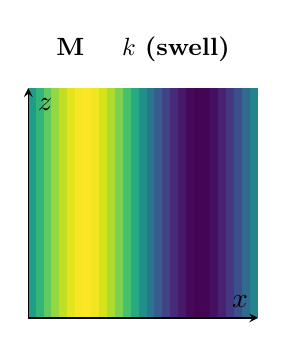
\begin{tikzpicture}
\begin{axis}[
    width=4.5cm, height=4.5cm,
    view={0}{90},
    xlabel={$x$}, ylabel={$z$},
    title={Μικρό $k$ (swell)},
    title style={font=\small\bfseries},
    colormap/viridis,
    colorbar=false,
    point meta min=-1, point meta max=1,
    axis lines=middle,
    ticks=none,
    enlargelimits=false
]
\addplot3[surf, shader=flat, samples=30, domain=0:4*pi, y domain=0:2*pi]
{sin(deg(0.5*x))};
\end{axis}
\end{tikzpicture}
\hspace{0.3cm}
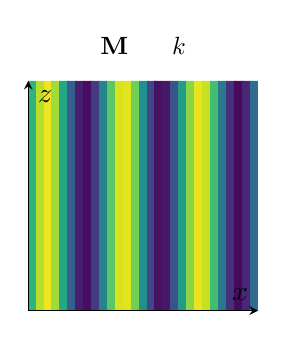
\begin{tikzpicture}
\begin{axis}[
    width=4.5cm, height=4.5cm,
    view={0}{90},
    xlabel={$x$}, ylabel={$z$},
    title={Μεσαίο $k$},
    title style={font=\small\bfseries},
    colormap/viridis,
    colorbar=false,
    point meta min=-1, point meta max=1,
    axis lines=middle,
    ticks=none,
    enlargelimits=false
]
\addplot3[surf, shader=flat, samples=30, domain=0:4*pi, y domain=0:2*pi]
{sin(deg(1.5*x))};
\end{axis}
\end{tikzpicture}
\hspace{0.3cm}
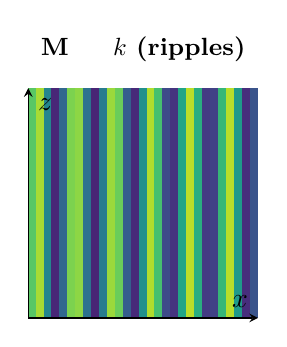
\begin{tikzpicture}
\begin{axis}[
    width=4.5cm, height=4.5cm,
    view={0}{90},
    xlabel={$x$}, ylabel={$z$},
    title={Μεγάλο $k$ (ripples)},
    title style={font=\small\bfseries},
    colormap/viridis,
    colorbar=false,
    point meta min=-1, point meta max=1,
    axis lines=middle,
    ticks=none,
    enlargelimits=false
]
\addplot3[surf, shader=flat, samples=30, domain=0:4*pi, y domain=0:2*pi]
{sin(deg(3*x))};
\end{axis}
\end{tikzpicture}
\caption{Κάτοψη της επιφάνειας της θάλασσας για διαφορετικούς κυματαριθμούς $k$.}
\label{fig:k_topview}
\end{figure}

Σημειώνεται ότι ο FFT αλγόριθμος Cooley--Tukey απαιτεί το μέγεθος του
πλέγματος να είναι δύναμη του δύο \(N = 2^m\) ώστε να μπορεί να διασπά
αναδρομικά έναν DFT μεγέθους \(N\) σε δύο μικρότερους DFT μεγέθους
\(N/2\).

\subsection{Φάσμα Phillips}\label{ux3c6ux3acux3c3ux3bcux3b1-phillips}

Αφού οριστούν οι διαθέσιμες κυματικές συνιστώσες, το επόμενο βήμα είναι
να καθοριστεί πόση ενέργεια αντιστοιχεί σε κάθε κύμα. Αυτό γίνεται μέσω
του φάσματος Phillips (Phillips 1957), μιας θεμελιώδους στατιστικής
προσέγγισης που εξακολουθεί να αποτελεί τη βάση για σύγχρονες μεθόδους
στα γραφικά (Horvath 2015).

Το φάσμα δίνεται από:

\[
P(\vec{k}) =
A
\cdot
\frac{e^{-1/(kL_w)^2}}{k^4}
\cdot
\cos^2\theta
\]

όπου \(A\) είναι σταθερά κλίμακας ενέργειας, \(L_w = V^2/g\) το
χαρακτηριστικό μήκος κύματος που σχετίζεται με την ταχύτητα ανέμου
\(V\), και \(\theta\) η γωνία μεταξύ του κυματικού διανύσματος και της
κατεύθυνσης του ανέμου.

Ο όρος \(1/k^4\) αυξάνει σημαντικά την ενέργεια των κυμάτων μεγάλου
μήκους κύματος, με αποτέλεσμα ο ωκεανός να κυριαρχείται από μεγάλα swell
waves αντί από μικρά ripples. Ο εκθετικός όρος \(e^{-1/(kL_w)^2}\)
λειτουργεί ως φίλτρο που αποκόπτει κύματα μεγαλύτερα από αυτά που μπορεί
να δημιουργήσει ο άνεμος. Για παράδειγμα, για άνεμο ταχύτητας
\(V=10\,\text{m/s}\), προκύπτει \(L_w \approx 10.2\,\text{m}\). Τέλος, ο
όρος \(\cos^2\theta\) εισάγει κατευθυντικότητα. Κύματα που κινούνται
παράλληλα προς τον άνεμο ενισχύονται, ενώ κύματα αντίθετης κατεύθυνσης
καταστέλλονται. Αν \(\hat{k}\) είναι το μοναδιαίο κυματικό διάνυσμα και
\(\hat{w}\) το μοναδιαίο διάνυσμα ανέμου, τότε:

\[
\cos\theta
=
\hat{k}\cdot\hat{w}
=
\frac{k_xw_x + k_zw_z}{k}
\]

και για \(\cos\theta \le 0\) θέτουμε \(P(\vec{k}) = 0\) ώστε να
απορρίπτονται κύματα που ταξιδεύουν αντίθετα από τον άνεμο.

\subsection{\texorpdfstring{Αρχικό φάσμα
\(h_0(\vec{k})\)}{Αρχικό φάσμα h\_0(\textbackslash vec\{k\})}}\label{ux3b1ux3c1ux3c7ux3b9ux3baux3cc-ux3c6ux3acux3c3ux3bcux3b1-h_0veck}

Το φάσμα Phillips καθορίζει μόνο τη στατιστική ενέργεια κάθε συχνότητας
και όχι τη συγκεκριμένη μορφή της θάλασσας. Για να παραχθεί μία μοναδική
αλλά στατιστικά σωστή επιφάνεια, εισάγονται τυχαίες φάσεις μέσω Gaussian
μεταβλητών.

Το αρχικό φάσμα Fourier ορίζεται ως:

\[
h_0(\vec{k})
=
\frac{\xi_1 + i\xi_2}{\sqrt{2}}
\sqrt{P(\vec{k})}
\]

όπου \(\xi_1,\xi_2 \sim \mathcal N(0,1)\) είναι ανεξάρτητες Gaussian
μεταβλητές.

\begin{figure}[htbp]
\centering
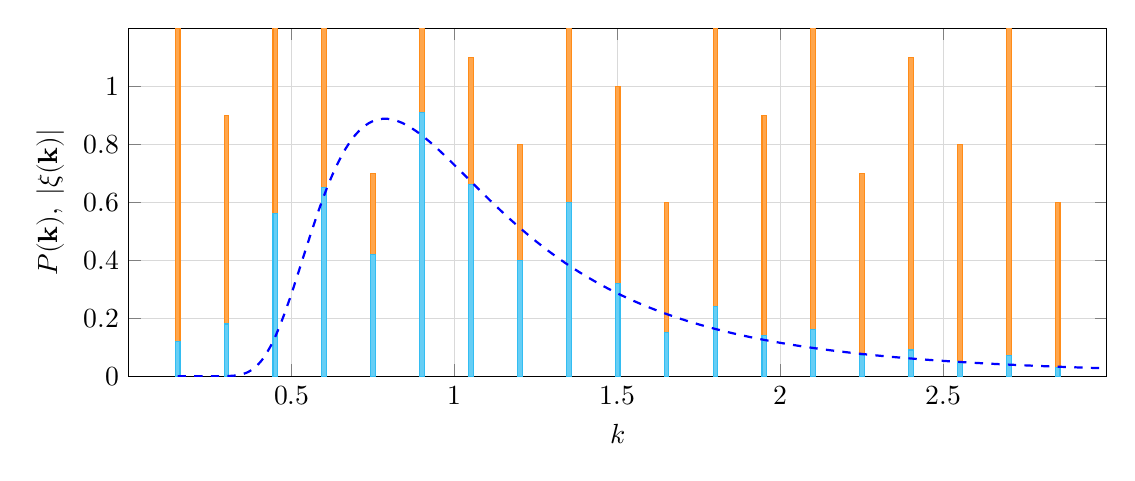
\begin{tikzpicture}
\begin{axis}[
    width=14cm,
    height=6cm,
    xlabel={$k$},
    ylabel={$P(\mathbf{k}),\; |\xi(\mathbf{k})|$},
    xmin=0, xmax=3,
    ymin=0, ymax=1.2,
    xtick={0.5, 1.0, 1.5, 2.0, 2.5},
    ytick={0, 0.2, 0.4, 0.6, 0.8, 1.0},
    grid=both,
    grid style={gray!30},
]

% --- Πορτοκαλί ράβδοι: τυχαίες τιμές |ξ(k)| ---
\addplot[
    ybar,
    bar width=0.06cm,
    fill=orange!70,
    draw=orange!90,
]
table[row sep=crcr] {
0.15 1.2 \\
0.30 0.9 \\
0.45 1.6 \\
0.60 1.3 \\
0.75 0.7 \\
0.90 1.4 \\
1.05 1.1 \\
1.20 0.8 \\
1.35 1.5 \\
1.50 1.0 \\
1.65 0.6 \\
1.80 1.2 \\
1.95 0.9 \\
2.10 1.3 \\
2.25 0.7 \\
2.40 1.1 \\
2.55 0.8 \\
2.70 1.4 \\
2.85 0.6 \\
};

% --- Γαλάζιες ράβδοι: |ξ(k)| * sqrt(P(k)) ---
\addplot[
    ybar,
    bar width=0.06cm,
    fill=cyan!60,
    draw=cyan!80,
]
table[row sep=crcr] {
0.15 0.12 \\
0.30 0.18 \\
0.45 0.56 \\
0.60 0.65 \\
0.75 0.42 \\
0.90 0.91 \\
1.05 0.66 \\
1.20 0.40 \\
1.35 0.60 \\
1.50 0.32 \\
1.65 0.15 \\
1.80 0.24 \\
1.95 0.14 \\
2.10 0.16 \\
2.25 0.07 \\
2.40 0.09 \\
2.55 0.05 \\
2.70 0.07 \\
2.85 0.03 \\
};

% --- Καμπύλη Phillips (κυανή) ---
\addplot[
    blue,
    thick,
    dashed,
    domain=0.15:3,
    samples=200,
]
{2.5*exp(-1/((x)*0.9)^2)/(x^4)};

\end{axis}
\end{tikzpicture}
\caption{Διαμόρφωση της τυχαιότητας από το φάσμα Phillips.}
\label{fig:phillips_random}
\end{figure}

Το σχήμα \ref{fig:phillips_random} αποτυπώνει οπτικά τη σχέση μεταξύ του
ντετερμινιστικού φάσματος Phillips και της στοχαστικής φύσης της
θάλασσας. Η κυανή διακεκομμένη καμπύλη αντιστοιχεί στο
\(P(\mathbf{k})\), δηλαδή στο αναμενόμενο ενεργειακό περιβάλλον κάθε
κυματικής συνιστώσας. Οι πορτοκαλί ράβδοι παριστάνουν τυχαίες τιμές
\(|\xi(\mathbf{k})|\), που προκύπτουν από ανεξάρτητες Gaussian
μεταβλητές και εισάγουν την απαραίτητη στοχαστικότητα. Όταν αυτές οι
τυχαίες τιμές πολλαπλασιαστούν με τη ρίζα του φάσματος
\(\sqrt{P(\mathbf{k})}\), προκύπτουν οι γαλάζιες ράβδοι, δηλαδή τα
πραγματικά πλάτη των κυμάτων \(|\xi(\mathbf{k})|\sqrt{P(\mathbf{k})}\).
Έτσι, το φάσμα Phillips λειτουργεί ως «καλούπι» που περιορίζει και
διαμορφώνει την τυχαιότητα, επιτρέποντας την παραγωγή ρεαλιστικών
επιφανειών που σέβονται τη στατιστική συμπεριφορά του ωκεανού
(Tessendorf 2001).

Η χρήση Gaussian κατανομής δεν είναι αυθαίρετη. Η επιφάνεια της θάλασσας
μπορεί να θεωρηθεί ως άθροισμα πολύ μεγάλου αριθμού ανεξάρτητων κυμάτων:

\[
h(x,z)
=
\sum_{i=1}^{M}
a_i
\cos(\vec{k}_i\cdot\vec{r}+\phi_i)
\]

και σύμφωνα με το Κεντρικό Οριακό Θεώρημα, όταν \(M \to \infty\), η
διαδικασία τείνει σε Gaussian κατανομή. Για τον λόγο αυτό και οι
συντελεστές Fourier θεωρούνται Gaussian. Για να προκύψει πραγματικό
πεδίο ύψους (height field) μετά τον αντίστροφο μετασχηματισμό Fourier,
απαιτείται το συνολικό φάσμα \(H(\vec{k},t)\) --- όπως θα οριστεί στην
επόμενη ενότητα --- να διαθέτει συζυγή (hermitian) συμμετρία:

\[
H^*(-\vec{k},t) = H(\vec{k},t)
\]

Η συνθήκη αυτή εξασφαλίζει ότι το τελικό πεδίο ύψους \(h(x,z,t)\)
παραμένει πραγματικό και όχι μιγαδικό και αποτελεί γενικό χαρακτηριστικό
όλων των διακριτών μετασχηματισμών Fourier πραγματικών σημάτων.
Σημειώνεται ότι η συμμετρία δεν επιβάλλεται στο ίδιο το αρχικό φάσμα: τα
\(h_0(\vec{k})\) και \(h_0(-\vec{k})\) επιλέγονται ανεξάρτητα.

\subsection{Χρονική
εξέλιξη}\label{ux3c7ux3c1ux3bfux3bdux3b9ux3baux3ae-ux3b5ux3beux3adux3bbux3b9ux3beux3b7}

Κάθε κυματική συνιστώσα εξελίσσεται ανεξάρτητα στον χρόνο. Για βαθιά
θάλασσα, η σχέση διασποράς δίνεται από:

\[
\omega(k)=\sqrt{gk}
\]

όπου \(g\) είναι η επιτάχυνση της βαρύτητας και \(k = |\vec{k}|\).

Η σχέση διασποράς \(\omega(k) = \sqrt{gk}\) είναι μη γραμμική και οδηγεί
στο φαινόμενο dispersion, δηλαδή στο γεγονός ότι κύματα διαφορετικού
μήκους ταξιδεύουν με διαφορετικές ταχύτητες. Αυτό είναι χαρακτηριστικό
της πραγματικής θαλάσσιας κίνησης.

Η χρονική εξέλιξη των συντελεστών Fourier δίνεται από:

\[
H(\vec{k},t)
=
h_0(\vec{k})e^{i\omega t}
+
h_0^*(-\vec{k})e^{-i\omega t}
\]

Ο δεύτερος όρος δεν είναι περιττός. Διατηρεί τη συζυγή (hermitian)
συμμετρία για κάθε χρονική στιγμή:

\[
H^*(-\vec{k},t)=H(\vec{k},t)
\]

ώστε μετά τον αντίστροφο FFT να προκύπτει πραγματική επιφάνεια νερού.

Αξίζει να τονιστεί ότι η συμμετρία αυτή δεν επιβάλλεται στις τυχαίες
μεταβλητές, αλλά προκύπτει εκ κατασκευής από το άθροισμα των δύο όρων:

\[
H^*(-\vec{k},t) = h_0^*(-\vec{k})\,e^{-i\omega t} + h_0(\vec{k})\,e^{i\omega t} = H(\vec{k},t).
\]

Αν αντίθετα επιβαλλόταν η συνθήκη \(h_0^*(-\vec{k}) = h_0(\vec{k})\)
απευθείας στο αρχικό φάσμα, οι δύο όροι θα συνδυάζονταν σε
\(2\,h_0(\vec{k})\cos(\omega t)\) και η επιφάνεια θα αποτελούνταν από
στάσιμα κύματα αντί για κύματα που ταξιδεύουν.

Έχοντας το \(H(\vec{k},t)\) για κάθε κελί του πλέγματος συχνοτήτων, το
πραγματικό ύψος της επιφάνειας στον φυσικό χώρο προκύπτει από τον
(αντίστροφο) μετασχηματισμό Fourier:

\[
h(x,z,t) = \sum_{\vec{k}} H(\vec{k},t)\, e^{i(k_xx+k_zz)},
\]

υπολογιζόμενο αποδοτικά μέσω 2D IFFT αντί για απευθείας άθροιση.

Το \(h(x,z,t)\) όμως περιγράφει μόνο την κατακόρυφη συνιστώσα του
κύματος --- ακριβώς το \(y(u,t)=A\cos(\cdot)\) που είχαμε δει στο
κεφάλαιο για τα κύματα Gerstner. Όπως όμως είχε φανεί εκεί, η ρεαλιστική
εικόνα ενός κύματος (αιχμηρές κορυφές, πλατιές κοιλάδες) απαιτεί και μια
οριζόντια μετατόπιση \(x(u,t)\). Η ίδια ιδέα μεταφέρεται εδώ στο πεδίο
συχνοτήτων: ο Tessendorf ορίζει ένα διανυσματικό πεδίο οριζόντιας
μετατόπισης

\[
\vec{D}(\vec{k},t) = i\,\frac{\vec{k}}{k}\,H(\vec{k},t),
\]

το οποίο μετασχηματίζεται κι αυτό με IFFT στον φυσικό χώρο, δίνοντας
\(\vec D(x,z,t)\). Κάθε σημείο του πλέγματος μετατοπίζεται τελικά στη
θέση \(\vec{x}+\vec{D}(x,z,t)\) αντί να μένει στην αρχική του
\(\vec{x}\) --- αναπαράγοντας έτσι, σε πλήρη 2D/φασματική μορφή, ακριβώς
το φαινόμενο της οριζόντιας εκτροπής που περιγράφτηκε αναλυτικά στο
κεφάλαιο Gerstner.

Το Σχήμα \ref{fig:choppy_displacement} δείχνει την επίδραση αυτή σε ένα
κύμα αποτελούμενο από λίγες συχνότητες (ανάλογο της υπέρθεσης
ημιτονοειδών της ενότητας «Άθροισμα συχνοτήτων», όχι ένα απλό ημίτονο):
η γκρι, διακεκομμένη καμπύλη είναι το ύψος \(h(x)\) χωρίς μετατόπιση,
ενώ η μπλε δείχνει το ίδιο κύμα αφού κάθε σημείο μετακινηθεί οριζόντια
κατά \(D(x)\) --- οι κορυφές γίνονται πιο αιχμηρές και οι κοιλάδες πιο
πλατιές, το χαρακτηριστικό ``choppy'' αποτέλεσμα.

\begin{figure}[htbp]
\centering
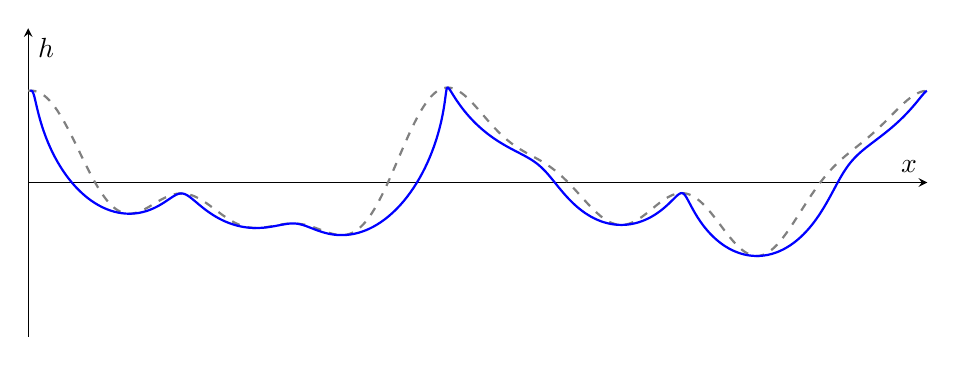
\begin{tikzpicture}
\begin{axis}[
  width=13cm, height=5.5cm,
  axis lines=middle,
  xlabel={$x$}, ylabel={$h$},
  xmin=0, xmax=12.6,
  ymin=-0.4, ymax=0.4,
  xtick=\empty, ytick=\empty,
  samples=400,
  domain=0:12.566
]
  % Χωρίς οριζόντια μετατόπιση: άθροισμα 3 αρμονικών h(x)
  \addplot[gray, dashed, thick]
    ({x},
     {0.15*cos(deg(x)) + 0.08*cos(deg(2*x+0.6)) + 0.04*cos(deg(3.5*x-1.0))});
 
  % Με οριζόντια μετατόπιση: παραμετρική καμπύλη (x+D(x), h(x))
  \addplot[blue, thick]
    ({x - 0.15*sin(deg(x)) - 0.16*sin(deg(2*x+0.6)) - 0.14*sin(deg(3.5*x-1.0))},
     {0.15*cos(deg(x)) + 0.08*cos(deg(2*x+0.6)) + 0.04*cos(deg(3.5*x-1.0))});
\end{axis}
\end{tikzpicture}
\caption{Κύμα με και χωρίς οριζόντια μετατόπιση $\vec D$.}
\label{fig:choppy_displacement}
\end{figure}

\section{Από τα μαθηματικά στον ψηφιακό
ωκεανό}\label{ux3b1ux3c0ux3cc-ux3c4ux3b1-ux3bcux3b1ux3b8ux3b7ux3bcux3b1ux3c4ux3b9ux3baux3ac-ux3c3ux3c4ux3bfux3bd-ux3c8ux3b7ux3c6ux3b9ux3b1ux3baux3cc-ux3c9ux3baux3b5ux3b1ux3bdux3cc}

Το άρθρο ξεκίνησε από ένα απλό ερώτημα: πώς μπορεί ένας υπολογιστής να
δημιουργήσει έναν πειστικό ψηφιακό ωκεανό; Η απάντηση δεν βρίσκεται μόνο
στην υπολογιστική ισχύ των σύγχρονων επεξεργαστών, αλλά κυρίως σε μια
αλυσίδα μαθηματικών ιδεών που αναπτύχθηκαν σταδιακά επί τρεις αιώνες. Τα
αναπτύγματα Taylor, ο τύπος του Euler, η θεωρία του Fourier και ο
γρήγορος μετασχηματισμός Fourier (FFT) συνθέτουν την αλυσίδα μαθηματικών
και υπολογιστικών ιδεών πάνω στην οποία στηρίζονται οι σύγχρονοι
αλγόριθμοι προσομοίωσης κυμάτων.

Η βασική ιδέα του Fourier, ότι κάθε πολύπλοκο σήμα μπορεί να αναλυθεί ως
άθροισμα απλούστερων ταλαντώσεων, δεν περιορίζεται στην προσομοίωση της
θάλασσας. Η ίδια μαθηματική αρχή αποτελεί θεμέλιο της επεξεργασίας ήχου
και εικόνας, της συμπίεσης δεδομένων, των τηλεπικοινωνιών, της ιατρικής
απεικόνισης, της σεισμολογίας καθώς και σε πλήθος άλλων εφαρμογών της
επιστήμης και της μηχανικής. Ο γρήγορος μετασχηματισμός Fourier (FFT)
κατέστησε εφικτή την αξιοποίηση αυτής της θεωρίας σε πραγματικές
εφαρμογές, επιτρέποντας την εκτέλεση υπολογισμών που διαφορετικά θα ήταν
πρακτικά αδύνατοι.

Την επόμενη φορά που θα παρακολουθήσουμε μια κινηματογραφική σκηνή με
φουρτουνιασμένη θάλασσα ή θα ταξιδέψουμε σε έναν ψηφιακό ωκεανό μέσα από
ένα βιντεοπαιχνίδι, ίσως αξίζει να θυμηθούμε ότι πίσω από κάθε κύμα δεν
κρύβεται μόνο η ισχύς της GPU, αλλά μια αλυσίδα μαθηματικών ιδεών που
ξεκινά από τον Taylor, περνά από τον Euler και τον Fourier και καταλήγει
στον FFT. Είναι μια όμορφη υπενθύμιση ότι ακόμη και οι πιο εντυπωσιακές
εικόνες της σύγχρονης ψηφιακής τεχνολογίας θεμελιώνονται σε μαθηματικές
ιδέες που διατυπώθηκαν πριν από αιώνες. Πίσω από κάθε ψηφιακό κύμα δεν
κρύβεται μόνο ένας αλγόριθμος· κρύβεται μια μαθηματική ιδέα.

\phantomsection\label{refs}
\begin{CSLReferences}{1}{0}
\bibitem[\citeproctext]{ref-ac4blackflag2013}
{``Assassin's Creed IV: Black Flag.''} 2013. Video game.

\bibitem[\citeproctext]{ref-bekesy1960}
Békésy, Georg von. 1960. \emph{Experiments in Hearing}. McGraw-Hill.

\bibitem[\citeproctext]{ref-burden2016}
Burden, Richard L., and J. Douglas Faires. 2016. \emph{Numerical
Analysis}. 10th ed. Cengage Learning.

\bibitem[\citeproctext]{ref-cooley1965}
Cooley, James W., and John W. Tukey. 1965. {``An Algorithm for the
Machine Calculation of Complex Fourier Series.''} \emph{Mathematics of
Computation} 19 (90): 297--301. \url{https://doi.org/10.2307/2003354}.

\bibitem[\citeproctext]{ref-crysis2007}
{``Crysis.''} 2007. Video game.

\bibitem[\citeproctext]{ref-fourier1822}
Fourier, Joseph. 1822. \emph{Th{é}orie Analytique de La Chaleur}. Paris:
Firmin Didot.

\bibitem[\citeproctext]{ref-fournier1986}
Fournier, Alain, and William T. Reeves. 1986. {``A Simple Model of Ocean
Waves.''} \emph{ACM SIGGRAPH Computer Graphics} 20 (4): 75--84.
\url{https://doi.org/10.1145/15886.15894}.

\bibitem[\citeproctext]{ref-gerstner1809}
Gerstner, Franz Joseph. 1809. {``Theorie Der Wellen.''}
\emph{Abhandlungen Der Königlichen Böhmischen Gesellschaft Der
Wissenschaften} 3: 1--24.

\bibitem[\citeproctext]{ref-horvath2015}
Horvath, Christopher J. 2015. {``Empirical Directional Wave Spectra for
Computer Graphics.''} In \emph{Proceedings of the 2015 Symposium on
Digital Production}, 29--39. DigiPro '15. New York, NY, USA: ACM.
\url{https://doi.org/10.1145/2791261.2791267}.

\bibitem[\citeproctext]{ref-lifeofpi2012}
{``Life of Pi.''} 2012. Motion picture.

\bibitem[\citeproctext]{ref-navier1822}
Navier, Claude-Louis. 1822. {``Mémoire Sur Les Lois Du Mouvement Des
Fluides.''} \emph{Mémoires de l'Académie Des Sciences de l'Institut de
France} 6: 389--440.

\bibitem[\citeproctext]{ref-phillips1957}
Phillips, O. M. 1957. {``On the Generation of Waves by Turbulent
Wind.''} \emph{Journal of Fluid Mechanics} 2 (5): 417--45.
\url{https://doi.org/10.1017/S0022112057000233}.

\bibitem[\citeproctext]{ref-seaofthieves2018}
{``Sea of Thieves.''} 2018. Video game.

\bibitem[\citeproctext]{ref-stokes1845}
Stokes, George Gabriel. 1845. {``On the Theories of the Internal
Friction of Fluids in Motion.''} \emph{Transactions of the Cambridge
Philosophical Society} 8: 287--319.

\bibitem[\citeproctext]{ref-taylor1715}
Taylor, Brook. 1715. \emph{Methodus Incrementorum Directa Et Inversa}.
London: William Innys.

\bibitem[\citeproctext]{ref-tessendorf2001}
Tessendorf, Jerry. 2001. {``Simulating Ocean Water.''}

\bibitem[\citeproctext]{ref-perfectstorm2000}
{``The Perfect Storm.''} 2000. Motion picture.

\bibitem[\citeproctext]{ref-titanic1997}
{``Titanic.''} 1997. Motion picture.

\bibitem[\citeproctext]{ref-waterworld1995}
{``Waterworld.''} 1995. Motion picture.

\end{CSLReferences}

\end{document}